\documentclass{article}
\usepackage[utf8]{inputenc}
\usepackage{graphicx}
\usepackage{amsmath }
\usepackage{amssymb}
\usepackage{subcaption}
\usepackage{float}
\usepackage{multirow}
\usepackage{nomencl}
\usepackage{bm}
\usepackage{hyperref}
\usepackage[makeroom]{cancel}
\usepackage{algorithm}
\usepackage{algorithmic}
\setcounter{section}{1}


\usepackage{cleveref} %referencing figures, equations and tables
\crefformat{figure}{Figure.~#2#1#3}
\crefformat{equation}{Eq.~#2#1#3}
\crefformat{table}{Table.~#2#1#3}
\crefformat{appendix}{Appendix.~#2#1#3}
\crefformat{section}{Section.~#2#1#3}

\title{A Review on \vspace{.2cm}\\ \huge \textbf{A Refined Sinusoidal Theory for Laminated Composite and Sandwich Plates} \vspace{.2cm}\\ \small Originally published by Ren Xiaohui, Wu Zhen \& Ji Bin}
\author{Amir Baharvand }
\date{}

\begin{document}

\maketitle

\makenomenclature

\nomenclature[A]{\textbf{CLPT}}{Classical Laminate Plate Theory}
\nomenclature[A]{\textbf{FSDT}}{First-order Shear Deformation plate Theory}
\nomenclature[A]{\textbf{RSPTZ}}{Refined sinusoidal shear deformation plate theory including the zig-zag function \\}

\nomenclature[L]{$M$}{Murakami's zig-zag function / Resultant moment}
\nomenclature[L]{$H$}{New zig-zag function}
\nomenclature[L]{$\bm{C}$}{Stiffness matrix}
\nomenclature[L]{$\bm{Q}$}{Transferred stiffness matrix}
\nomenclature[L]{$E$}{Young's modulus}
\nomenclature[L]{$Z$}{Ply coordinate along $z$-axis / Zig-zag function}
\nomenclature[L]{$N$}{Zig-zag parameter / Resultant force}
\nomenclature[L]{$a$}{Length / Zig-zag parameter}
\nomenclature[L]{$b$}{Width / Zig-zag parameter}
\nomenclature[L]{$h$}{Thickness}
\nomenclature[L]{$u$}{Displacement along $x$-axis}
\nomenclature[L]{$v$}{Displacement along $y$-axis}
\nomenclature[L]{$w$}{Displacement along $z$-axis}
\nomenclature[L]{$U$}{Displacement coefficients in Navier's solution along $x$-axis / Strain energy}
\nomenclature[L]{$V$}{Displacement coefficients in Navier's solution along $y$-axis}
\nomenclature[L]{$W$}{Displacement coefficients in Navier's solution along $z$-axis}
\nomenclature[L]{$q$}{Transverse distributed load}
\nomenclature[L]{$p$}{In-plane distributed load}
\nomenclature[L]{$T$}{Axial load / Transverse shear traction}
\nomenclature[L]{$W$}{Work}
\nomenclature[L]{$V$}{Resultant shear force}
\nomenclature[L]{$\bm{K}$}{Matrix of equations}
\nomenclature[L]{$\bm{d}$}{Displacement vector}
\nomenclature[L]{$\bm{p}$}{Load vector}
\nomenclature[L]{$n$}{Number of terms in Navier's solution / Normal vector}
\nomenclature[L]{$m$}{Number of terms in Navier's solution}
\nomenclature[L]{$ds$}{Infinitesimal element}
\nomenclature[L]{$\overline{N}$}{Secondary boundary condition (resultant force)}
\nomenclature[L]{$\overline{M}$}{Secondary boundary condition (resultant moment)}
\nomenclature[L]{$\overline{V}$}{Secondary boundary condition (resultant shear force)}
\nomenclature[L]{$x$}{$x$-axis}
\nomenclature[L]{$y$}{$y$-axis}
\nomenclature[L]{$z$}{$z$-axis}

\nomenclature[S]{$x$}{$x$-axis in coordinate system}
\nomenclature[S]{$y$}{$y$-axis in coordinate system}
\nomenclature[S]{$z$}{$z$-axis in coordinate system / Zig-zag}
\nomenclature[S]{$1$}{$x$-axis in lamina coordinate system / Sinusoidal function shear displacement coefficient / Label for $\phi$ functions in strain-displacement / Laminate bottom surface coordinate in $z$-direction}
\nomenclature[S]{$2$}{$y$-axis in lamina coordinate system / Label for $\phi$ functions in strain-displacement}
\nomenclature[S]{$3$}{$z$-axis in lamina coordinate system / Label for $\phi$ functions in strain-displacement}
\nomenclature[S]{$s$}{Shear}
\nomenclature[S]{$b$}{Bending / Bottom}
\nomenclature[S]{$k$}{Ply number}
\nomenclature[S]{$0$}{Mid-plane}
\nomenclature[S]{$t$}{Top}
\nomenclature[S]{$N$}{Laminate top surface coordinate in $z$-direction}
\nomenclature[S]{$T$}{Transpose}

\nomenclature[G]{$\theta$}{Angle}
\nomenclature[G]{$\sigma$}{Normal stress}
\nomenclature[G]{$\tau$}{Shear stress}
\nomenclature[G]{$\epsilon$}{Normal strain}
\nomenclature[G]{$\gamma$}{Shear strain}
\nomenclature[G]{$\zeta$}{Zig-zag parameter}
\nomenclature[G]{$\mu$}{Shear modulus}
\nomenclature[G]{$\nu$}{Poisson's ratio}
\nomenclature[G]{$\Omega$}{Plate area}
\nomenclature[G]{$\Gamma$}{Plate boundary}
\nomenclature[G]{$\delta$}{Variational}

\printnomenclature
\tableofcontents

\section*{Abstract}
A refined sinusoidal theory for composite laminates using a new zig-zag function \cite{Xiaohui2020} is proposed which automatically satisfies the traction-free boundary conditions on the top and bottom surfaces of the laminate. Next, equilibrium equations are obtained using the principle of virtual displacement and the Navier's solution is invoked to solve the boundary value problem. Analytic results are compared to the exact solution from three-dimensional elasticity [2], classical and first-order shear deformation theories for laminated composites. The present theory is capable of calculating displacement and stress fields with excellent accuracy.

\section{Introduction}
Composites are widely used in industry, specifically aerospace applications where composites offer the appealing strength-to-weight ratio. Compared to good in-planes modulus, composites are susceptible to transverse loading due to their weak transverse modulus. For example, for a typical wind turbine blade, the ratio of the transverse shear modulus to the in-plane shear modulus is about 0.1; therefore, the determination of transverse shear stresses is of paramount importance when analyzing composite laminates. \\

The isotropic one-layer plate theories are not able to characterize the piecewise (zig-zag) behavior of displacements and stresses in composite laminates \cite{Carrera2003}. First-order shear deformation theories lack accuracy due to high dependency on the selected shear correction factor. Furthermore, the shear strains are assumed constant along the thickness of the plate.
Despite the success of higher-order shear deformation theories in yielding accurate results, layer-wise theories have been introduced in which displacements and stresses are calculated for every single layer. The major drawback of layer-wise theories is the dependency of computation on degrees of freedom of the laminate which rises by increasing the number of layups \cite{Li1995}. \\

In order to utilize the advantages of layer-wise theories and to reduce the computational cost, a combination of higher-order shear deformation along with layer-wise theories have been introduced to describe the piecewise transverse displacement and stress of composite laminates. It is shown that the use of a zig-zag function is more effective than increasing the order of in-plane and transverse displacement components in higher-order theories \cite{Carrera2004}.\\

The present report replicates the result of a refined sinusoidal plate theory using a new zig-zag function by Xiaohui \emph{et al.} \cite{Xiaohui2020} which is inspired upon Touratier \cite{Touratier1991} sinusoidal shear deformation and Murakami's zig-zag function \cite{Murakami1986}. 

\section{The Proposed Zig-Zag Function}
One of the difficulties in characterizing displacements in composite laminates is the rapid change of in-plane displacements, usually due to stacking sequence. An efficient approach to overcome the abovementioned problem, as reported in the literature \cite{Carrera2004}, is to combine the sinusoidal shear deformation theory with a zig-zag function, \emph{e.g.}, Murakami's zig-zag function, to create the piecewise behavior in the in-plane displacement. A zig-zag function, $Z^k(z)$, is usually defined as 

\begin{equation}
    Z^k(z) = (-1)^k f(\zeta_k)
    \label{eq:zigzag}
\end{equation}

where

\begin{equation*}
    \begin{matrix}
    \zeta_k = a_k z - b_k & , 
     a_k = \frac{2}{z_{k+1} - z_k} & , 
     b_k = \frac{z_{k+1} + z_k}{z_{k+1} - z_k} & 
    \end{matrix}
\end{equation*}

$z_k$ and $z_{k+1}$ denote the lower and upper coordinates of $k$-th layer demonstrated in \cref{fig:laminate}. \\

\begin{figure}[H]
    \centering
    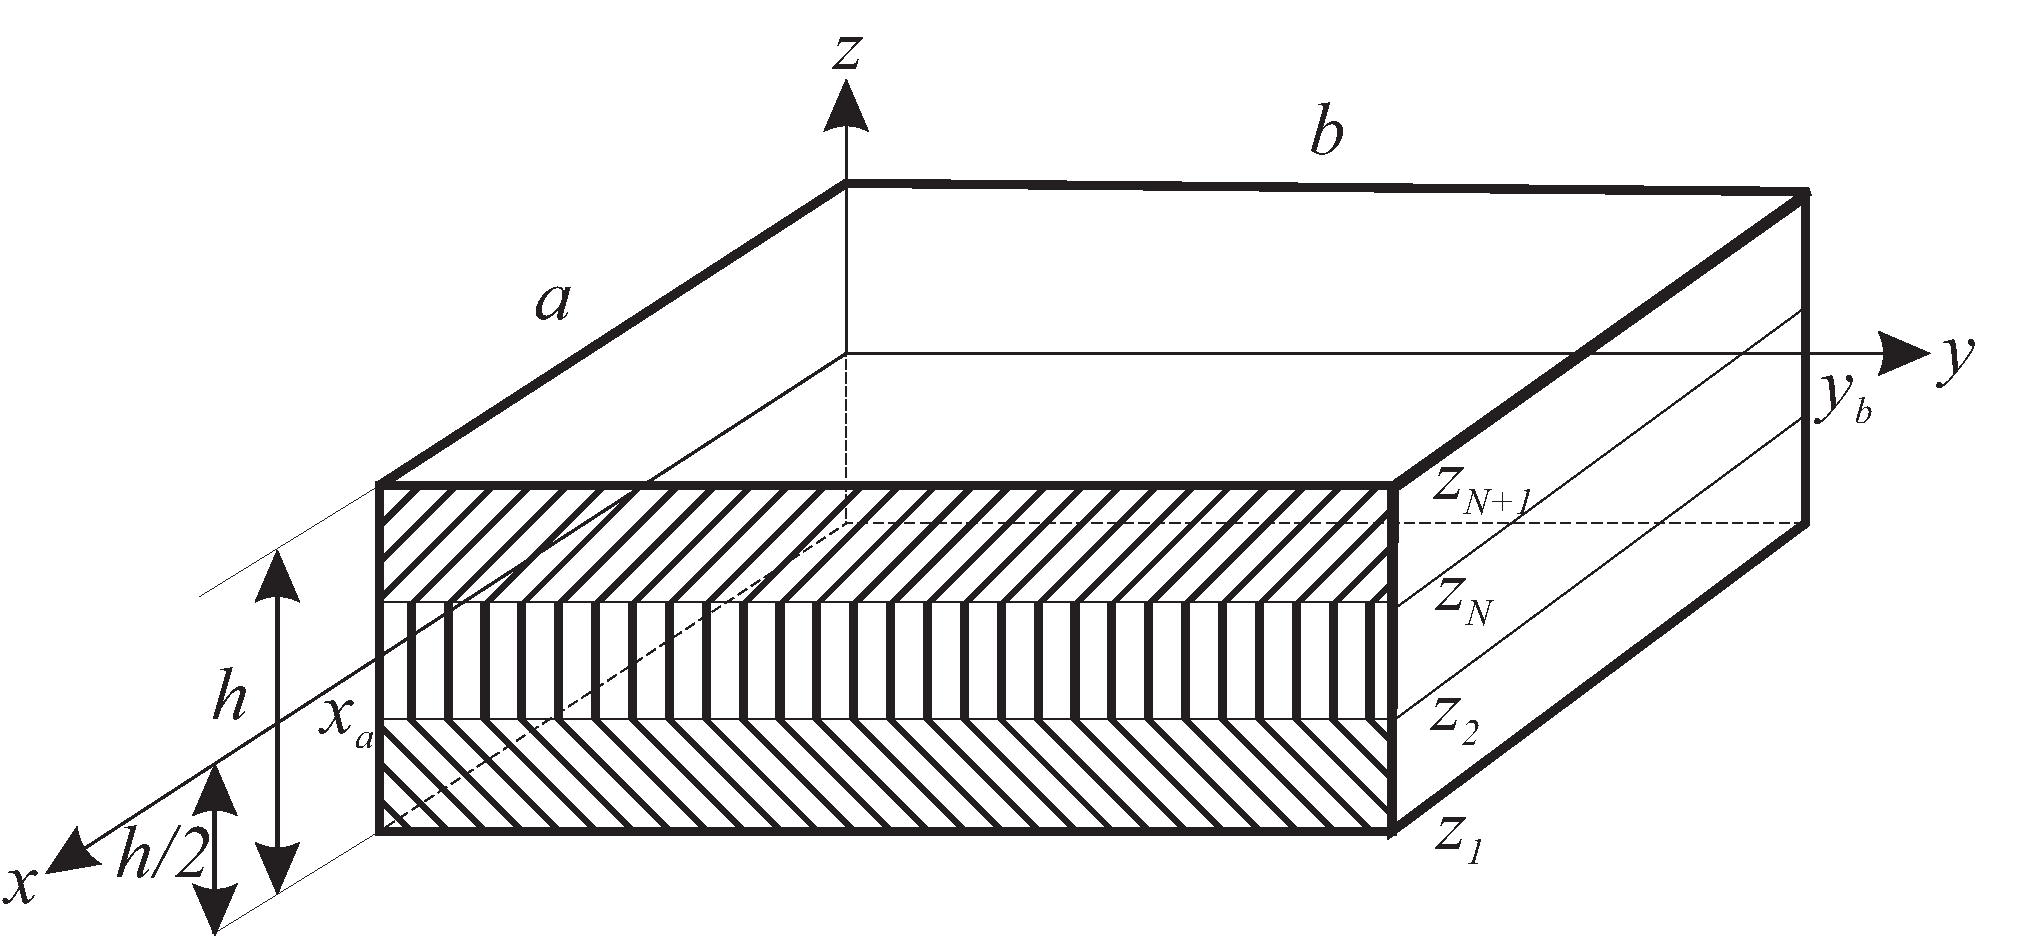
\includegraphics[width = 0.8\textwidth ]{figures/laminate.pdf}
    \caption{A Schematic of a composite laminate and the coordinate system.}
    \label{fig:laminate}
\end{figure}

The Murakami's zig-zag function, $M^k(z)$, is obtained by setting $f(\zeta_k)=\zeta_k$ and is given as

\begin{equation}
    M^k(z) = (-1)^k \zeta_k
    \label{eq:murakami}
\end{equation}

where $\zeta_k$ is defined according to \cref{eq:zigzag}. \cref{eq:murakami} indicates a linear distribution function through the plate thickness (\cref{fig:HM}). The main drawback of the Murakami's function is the violation of the traction-free boundary condition on the top and bottom surfaces of the laminate. \cref{fig:dMH} shows the derivative of $M^k(z)$ w.r.t $z$ where the zero transverse shear condition is clearly violated on the top and bottom surfaces. Hence, a new zig-zag function, $H^k(z)$, is proposed which satisfies a priori the zero boundary conditions on the top and bottom surfaces. \\

In the $H^k(z)$ function, $f(\zeta_k)$ is replaced with a $\sinh(\zeta_k)$ function accompanied by two other terms, as given in \cref{eq:Hzigzag} (see \cref{app:H-email} for a comment on $H^k(z)$ terms)

\begin{equation}
    H^k(z) = N^k(z) + N^k_1(z) + N^k_N(z)
    \label{eq:Hzigzag}
\end{equation}

where

\begin{align*}
    & N^k(z) = (-1)^k \sinh(\zeta_k) \\
    & N^k_1(z) = -(z^2 / 2 / z_1 + (z^3 -1.5z_1 z^2) / 6 / z^2_{N+1})(-a_1\cosh(-1)) \\
    & N^k_N(z) = -((z^3 - 1.5z_1 z^2) / 6 / z^2_{N+1})((-1)^N a_N \cosh(1))
\end{align*}

$a_1$, $a_N$ and $\zeta_k$ can be calculated from \cref{eq:zigzag}. $z_1$ to $z_{N+1}$ are the coordinates of each layer in the $z$-direction as demonstrated in \cref{fig:laminate}. $H^k(z)$ is plotted for a three-layer composite laminate in \cref{fig:HM}. While $M^k(z)$ varies linearly through each layer, $H^k(z)$ utilizes a nonlinear distribution to provide a better insight into the in-plane displacements at each layer. The derivative of $H^k(z)$ w.r.t $z$ is plotted in \cref{fig:dMH}. As it can be seen, $H^k(z)$ is able to fulfill the zero boundary conditions on the top and bottom surfaces.

\begin{figure}[H]
        \begin{subfigure}{0.5\textwidth}
            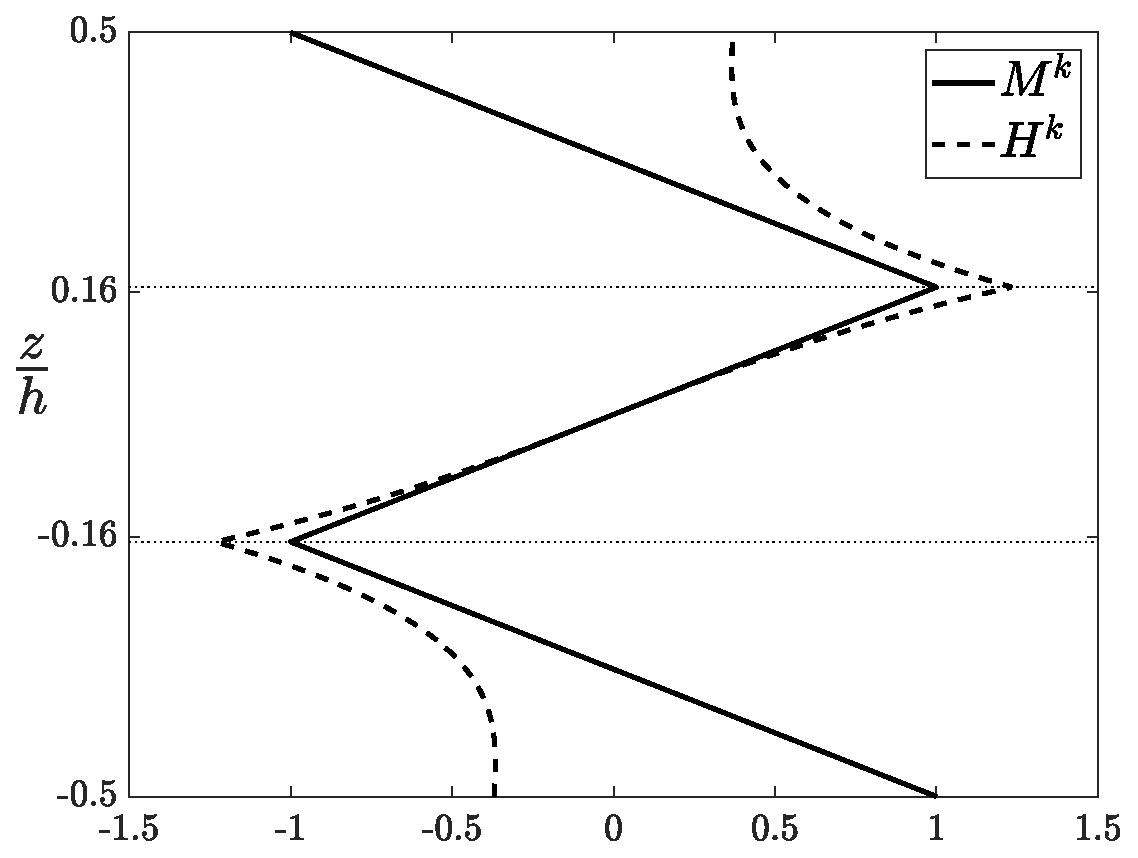
\includegraphics[width=1\linewidth, height=0.8\linewidth]{figures/MzHz.eps} 
            \caption{}
            \label{fig:HM}
        \end{subfigure}
        \begin{subfigure}{0.5\textwidth}
            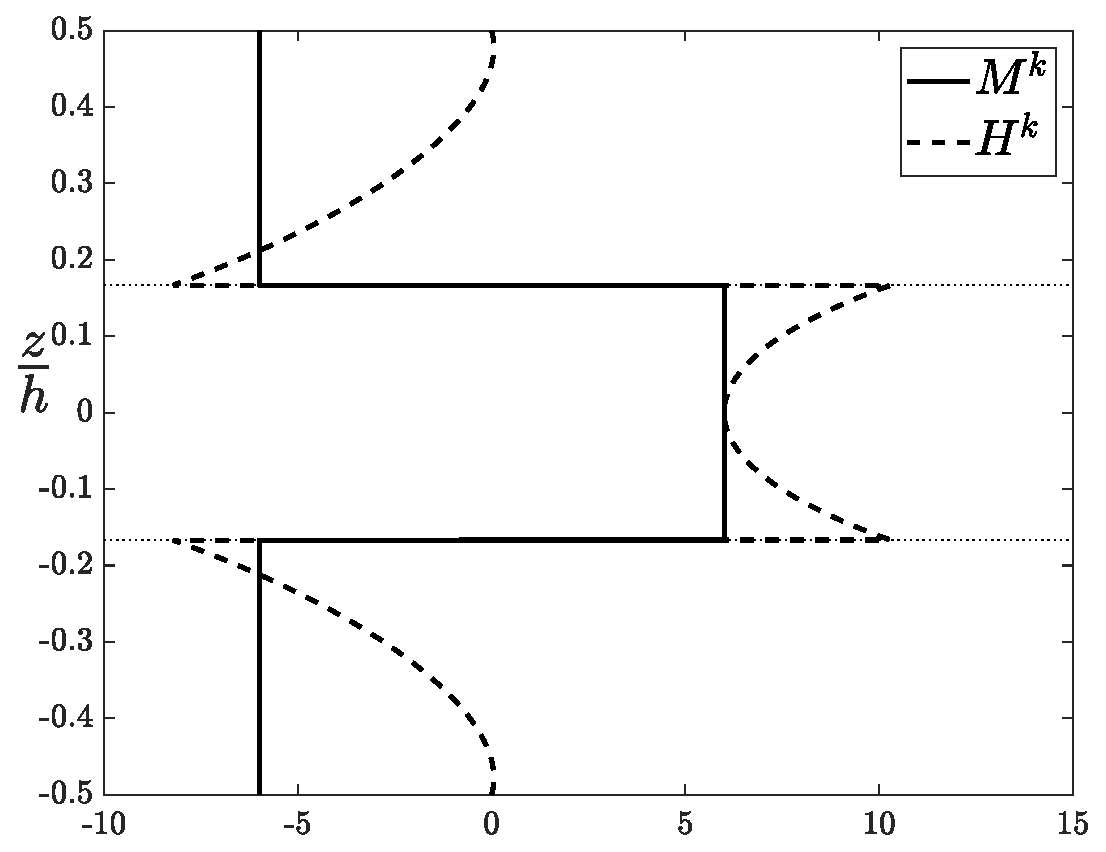
\includegraphics[width=1\linewidth, height=0.8\linewidth]{figures/dMzdHz.eps} 
            \caption{}
            \label{fig:dMH}
        \end{subfigure}
    \caption{Comparison of (a) $M^k(z)$ and $H^k(z)$ functions and (b) derivatives of $M^k(z)$ and $H^k(z)$ functions.}
    % \label{}
\end{figure}

\section{The Theory}
\subsection{Assumptions}
In developing the proposed theory, it is assumed that there is no elongation in the transverse direction and strains are infinitesimal.

\subsection{Displacement Fields}
Displacement fields are borrowed from a five-unknown shear deformation theory and combined with the zig-zag function displacement field. The general form of the displacement fields can be written as

\begin{gather}
    u^k = u_0 + u_b + u_s + u_z^k \notag\\
    v^k = v_0 + v_b + v_s + v_z^k \notag\\
    w = w_0
\end{gather}

where $u^k$, $v^k$ are the in-plane displacements and $w$ is the transverse displacement. $u_0$, $v_0$ and $w_0$ are the corresponding mid-plane displacements. $u_b$ and $v_b$ are the bendings, $u_s$ and $v_s$ are the shear displacements. Finally, $u_z^k$ and $v_z^k$ are the zig-zag displacement components. The expression for each of the abovementioned displacement fields is provided below. 

\begin{equation*}
    \begin{matrix}
    u_b = -z \displaystyle\frac{\partial w_0}{\partial x} & , 
    v_b = -z \displaystyle\frac{\partial w_0}{\partial y} & , 
    u_s = \displaystyle\frac{h}{\pi} \sin \left (\displaystyle\frac{\pi z}{h} \right ) u_1 & ,
    v_s = \displaystyle\frac{h}{\pi} \sin \left (\displaystyle\frac{\pi z}{h} \right ) v_1
    \end{matrix}
\end{equation*}

\begin{equation*}
    \begin{matrix}
    u_z^k = H^k(z) u_z &, 
    v_z^k = H^k(z) v_z
    \end{matrix}
\end{equation*}

As it can be seen from equations, the zig-zag displacement components are the only layer-dependent variables.

\subsection{Strain-Displacement Relation}
Assuming infinitesimal strains, the strain-displacement relations can be written as 

\begin{flalign*}
    & \epsilon^k_{x} = \frac{\partial u^k}{\partial x}  = \frac{\partial u_0}{\partial x} + \phi_1 \frac{\partial u_1}{\partial x} + \phi_2 \frac{\partial u_z}{\partial x} + \phi_3 \frac{\partial ^2w_0}{\partial x^2} & \notag\\
    & \epsilon^k_{y} = \frac{\partial v^k}{\partial y}  = \frac{\partial v_0}{\partial y} + \phi_1 \frac{\partial v_1}{\partial y} + \phi_2 \frac{\partial v_z}{\partial y} + \phi_3 \frac{\partial ^2w_0}{\partial y^2} & \notag\\
     & \gamma^k_{xy} = \frac{\partial u^k}{\partial y}  \frac{\partial v^k}{\partial x}  = \frac{\partial u_0}{\partial y} + \phi_1 \frac{\partial u_1}{\partial y} + \phi_2 \frac{\partial u_z}{\partial y} + \frac{\partial v_0}{\partial x} + \phi_1 \frac{\partial v_1}{\partial x} + \phi_2 \frac{\partial v_z}{\partial x} + 2 \phi_3 \frac{\partial ^2w_0}{\partial x \partial y} & \notag \\
     & \gamma^k_{xz} = \frac{\partial u_s}{\partial z}  \frac{\partial u_z^k}{\partial z} = \cos \left (\displaystyle\frac{\pi z}{h} \right ) u_1 + \frac{\partial H^k(z)}{\partial z} u_z = \dfrac{\partial \phi_1}{\partial z} u_1 + \dfrac{\partial \phi_2}{\partial z} u_z  & \notag \\
     & \gamma^k_{yz} = \frac{\partial v_s}{\partial z}  \frac{\partial v_z^k}{\partial z} = \cos \left (\displaystyle\frac{\pi z}{h} \right ) v_1 + \frac{\partial H^k(z)}{\partial z} v_z = \dfrac{\partial \phi_1}{\partial z} v_1 + \dfrac{\partial \phi_2}{\partial z} v_z & 
\end{flalign*}

where 

\begin{equation*}
    \begin{matrix}
    \phi_1 = \displaystyle\frac{h}{\pi} \sin \left (\displaystyle\frac{\pi z}{h} \right ) &, 
    \phi_2 = H^k(z) &,
    \phi_3 = -z
    \end{matrix}
\end{equation*}

One may easily identify the zero shear strains on the top and bottom surfaces of the laminate from the definition of transverse shear strains, $\gamma^k_{xz}$ and $\gamma^k_{yz}$.

\subsection{The Principle of Virtual Displacement}
\cref{fig:loading} illustrates the applied loading and boundary condition along with the coordinate system and geometry of the composite laminate. $p^b(x, y)$ and $p^t(x, y)$ are the in-plane distributed loads. Superscript $b$ and superscript $t$ denote the bottom and top surfaces. $q^b(x, y)$ and $q^t(x, y)$ are the transverse loads. $T_{x_0}$, $T_{x_a}$, $T_{y_0}$ and $T_{y_b}$ are the axial loads and $T_{{xz}_0}$, $T_{{xz}_a}$, $T_{{yz}_0}$ and $T_{{yz}_b}$ are the transverse shear tractions at the cross-section $x=0$, $x=a$, $y=0$ and $y=b$, respectively. \\

Applying the principle of virtual displacement for the plate shown in \cref{fig:loading} under static condition gives

\begin{equation}
    \delta U - \delta W = 0
    \label{eq:wvp}
\end{equation}

where $\delta U$ is the strain energy and $\delta W$ is the work done by external forces. The integral domain is defined on $\Omega \times (\dfrac{-h}{2}, \dfrac{h}{2})$ and $\Gamma$ is the boundary embracing the circumference of the plate. $\Omega$ and $h$ are the plate area and thickness, respectively. 

\begin{figure}[ht]
    \centering
    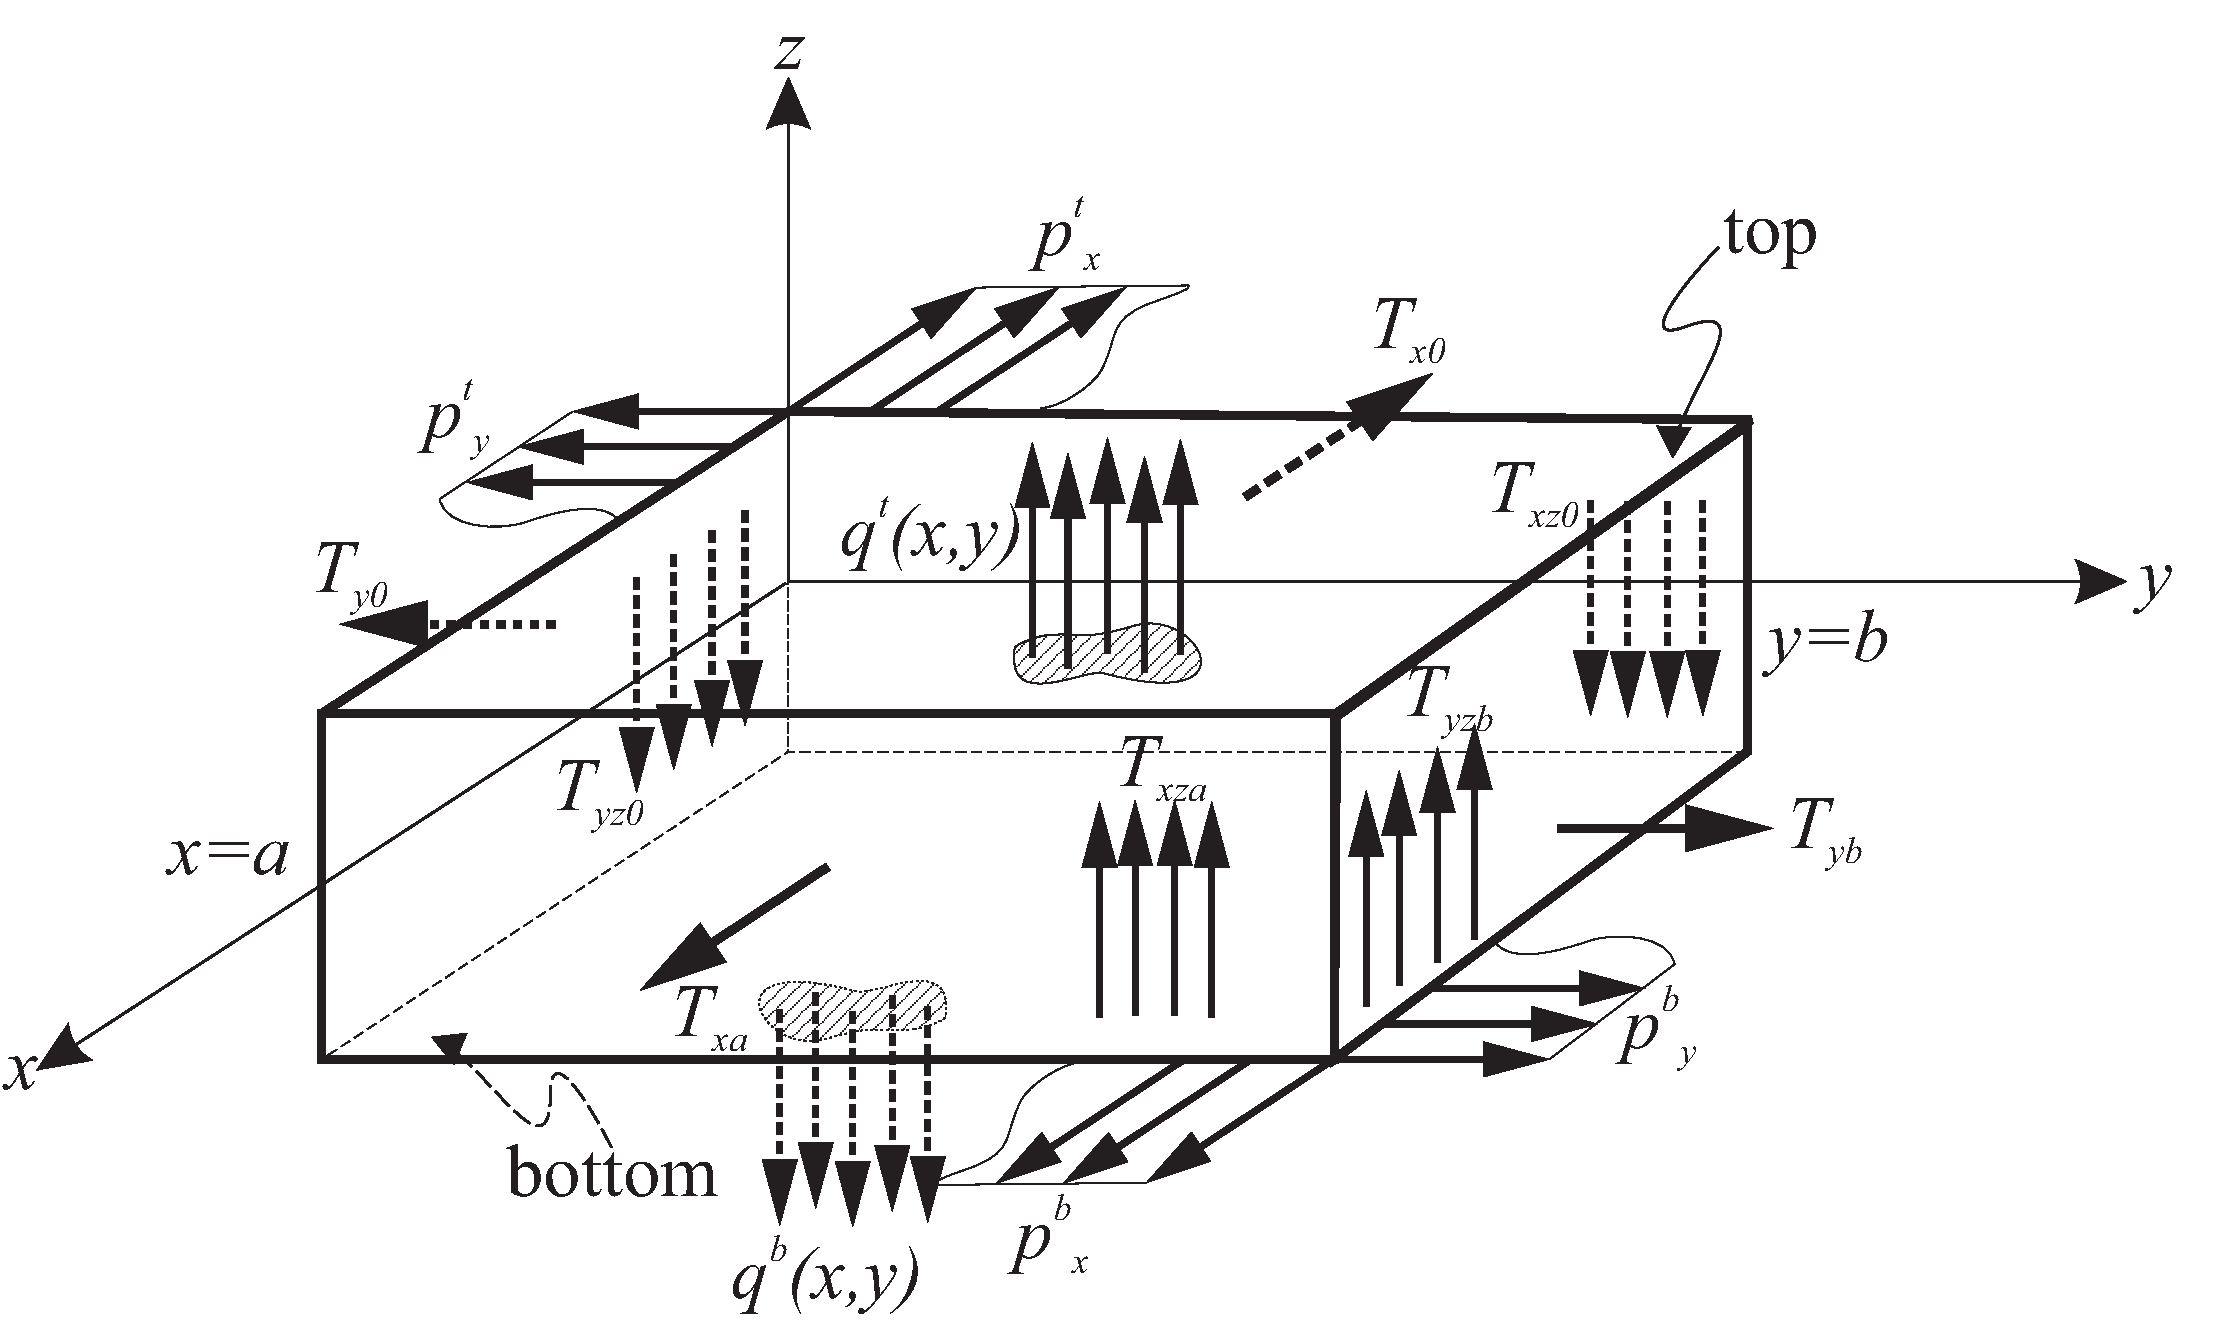
\includegraphics[width = 0.8\textwidth ]{figures/loading.pdf}
    \caption{Plate applied loading, boundary conditions, geometry and coordinate system (plies are not shown).}
    \label{fig:loading}
\end{figure}

\subsubsection{Strain Energy}\label{sec:strain_energy}
The virtual strain energy is given  as

\begin{flalign}
    \delta U =  \int_{\Omega} \int_{-\frac{h}{2}}^{\frac{h}{2}} &( 
    \sigma_x^k \delta \epsilon_x^k + \sigma_y^k \delta \epsilon_y^k + \tau_{yz}^k \delta \gamma_{yz}^k + \tau_{zx}^k \delta \gamma_{zx}^k + \tau_{xy}^k \delta \gamma_{xy}^k
    ) dz dx dy  &\notag \\
    = \int_{\Omega} \int_{-\frac{h}{2}}^{\frac{h}{2}} & \Bigg( \Bigg. 
    \sigma_x^k \frac{\partial \delta u_0}{\partial x} + \sigma_x^k \phi_1 \frac{\partial \delta u_1}{\partial x} + \sigma_x^k \phi_2 \frac{\partial \delta u_z}{\partial x} + \sigma_x^k \phi_3 \frac{\partial^2 \delta w_0}{\partial x^2}  &\notag\\
    & + \sigma_y^k \frac{\partial \delta v_0}{\partial y} + \sigma_y^k \phi_1 \frac{\partial \delta v_1}{\partial y} + \sigma_y^k \phi_2 \frac{\partial \delta v_z}{\partial y} + \sigma_y^k \phi_3 \frac{\partial^2 \delta w_0}{\partial y^2} &\notag \\
    & + \tau_{yz}^k \frac{\partial \phi_1}{\partial z} \delta v_1 + \tau_{yz}^k \frac{\partial \phi_2}{\partial z} \delta v_z + \tau_{xz}^k \frac{\partial \phi_1}{\partial z} \delta u_1 + \tau_{xz}^k \frac{\partial \phi_2}{\partial z} \delta u_z  &\notag\\
    & + \tau_{xy}^k \frac{\partial \delta u_0}{\partial y} + \tau_{xy}^k \phi_1 \frac{\partial \delta u_1}{\partial y} + \tau_{xy}^k \phi_2 \frac{\partial \delta u_z}{\partial y} +
    \tau_{xy}^k \frac{\partial \delta v_0}{\partial x}  &\notag\\
    & + \tau_{xy}^k \phi_1 \frac{\partial \delta v_1}{\partial x} + \tau_{xy}^k \phi_2 \frac{\partial \delta v_z}{\partial x} +
    2 \tau_{xy}^k \phi_3 \frac{\partial^2 \delta w_0}{\partial x \partial y}
    \Bigg. \Bigg) dz dx dy
    \label{delU}
\end{flalign}

By replacing stresses in the form of resultant forces and moments according to the set of equations in \cref{eq:resultant}, \cref{delU} can be rewritten in the form of \cref{delU_final}.

\begin{equation}
\begin{matrix}
    \begin{Bmatrix}
            N_x \\
            M_{x1} \\
            M_{x2} \\
            M_{x3} \\
    \end{Bmatrix} = 
    \displaystyle\int_{-\frac{h}{2}}^{\frac{h}{2}}
    \begin{Bmatrix}
            \sigma_x^k \\
            \sigma_x^k \phi_1 \\
            \sigma_x^k \phi_2 \\
            \sigma_x^k \phi_3 \\
    \end{Bmatrix}
    dz,
    \begin{Bmatrix}
            N_y \\
            M_{y1} \\
            M_{y2} \\
            M_{y3} \\
    \end{Bmatrix} = 
    \displaystyle\int_{-\frac{h}{2}}^{\frac{h}{2}}
    \begin{Bmatrix}
            \sigma_y^k \\
            \sigma_y^k \phi_1 \\
            \sigma_y^k \phi_2 \\
            \sigma_y^k \phi_3 \\
    \end{Bmatrix}
    dz,
        \begin{Bmatrix}
            V_{x1} \\
            V_{x2} \\
    \end{Bmatrix} = 
    \displaystyle\int_{-\frac{h}{2}}^{\frac{h}{2}}
    \begin{Bmatrix}
            \displaystyle\frac{\partial \phi_1}{\partial z}\tau_{xz}^k \\
            \displaystyle\frac{\partial \phi_2}{\partial z}\tau_{xz}^k \\
    \end{Bmatrix}
    dz
\end{matrix}
\label{eq:resultant}
\end{equation}

\begin{equation*}
\begin{matrix}
        \begin{Bmatrix}
            V_{y1} \\
            V_{y2} \\
    \end{Bmatrix} = 
    \displaystyle\int_{-\frac{h}{2}}^{\frac{h}{2}}
    \begin{Bmatrix}
            \displaystyle\frac{\partial \phi_1}{\partial z}\tau_{yz}^k \\
            \displaystyle\frac{\partial \phi_2}{\partial z}\tau_{yz}^k \\
    \end{Bmatrix}
    dz,
    \begin{Bmatrix}
            N_{xy} \\
            M_{xy1} \\
            M_{xy2} \\
            M_{xy3} \\
    \end{Bmatrix} = 
    \displaystyle\int_{-\frac{h}{2}}^{\frac{h}{2}}
    \begin{Bmatrix}
            \tau_{xy}^k \\
            \tau_{xy}^k \phi_1 \\
            \tau_{xy}^k \phi_2 \\
            \tau_{xy}^k \phi_3 \\
    \end{Bmatrix}
    dz
\end{matrix}
\end{equation*}

\begin{flalign}
    \delta U = \int_{\Omega} \int_{-\frac{h}{2}}^{\frac{h}{2}} & \Bigg( \Bigg. 
    N_x \frac{\partial \delta u_0}{\partial x} + M_{x1} \phi_1 \frac{\partial \delta u_1}{\partial x} + M_{x2} \frac{\partial \delta u_z}{\partial x} + M_{x3} \frac{\partial^2 \delta w_0}{\partial x^2}  &\notag\\
    & + N_y \frac{\partial \delta v_0}{\partial y} + M_{y1} \frac{\partial \delta v_1}{\partial y} + M_{y2} \frac{\partial \delta v_z}{\partial y} + M_{y3} \frac{\partial^2 \delta w_0}{\partial y^2} &\notag \\
    & + V_{y1} \delta v_1 + V_{y2} \delta v_z + V_{x1} \delta u_1 + V_{x2} \delta u_z  &\notag\\
    & + N_{xy} \frac{\partial \delta u_0}{\partial y} + M_{xy1} \frac{\partial \delta u_1}{\partial y} + M_{xy2} \frac{\partial \delta u_z}{\partial y} +
    N_{xy} \frac{\partial \delta v_0}{\partial x} + M_{xy1} \frac{\partial \delta v_1}{\partial x} + M_{xy2} \frac{\partial \delta v_z}{\partial x} &\notag \\
    & + 2 M_{xy3} \frac{\partial^2 \delta w_0}{\partial x \partial y}
    \Bigg. \Bigg) dz dx dy
    \label{delU_final}
\end{flalign}

The complete derivation of $\delta U$ is given in \cref{app:delU}.

\subsubsection{External Work}\label{sec:virtual_work}
The virtual work by external forces can be written as  

\begin{flalign}
    \delta W = \delta W_{px} + \delta W_{py} + \delta W_{q} + \delta W_{T_{x0}} + \delta W_{T_{y0}} + \delta W_{T_{xa}} + \delta W_{T_{yb}} 
    \label{delW}
\end{flalign}

where,

\begin{flalign*}
    &\delta W_{px} = -\int_{\Omega} \left [ p_x^b \delta u_0^1 (x, y, z_1) + p_x^t \delta u_0^N (x, y, z_{N+1}) \right] dxdy \\
    &\delta W_{py} = -\int_{\Omega} \left [ p_y^b \delta v_0^1 (x, y, z_1) + p_y^t \delta v_0^N (x, y, z_{N+1}) \right] dxdy \\
    &\delta W_{q} = -\int_{\Omega} \left [ q^b \delta w (x, y, z_1) + p_y^t \delta w (x, y, z_{N+1}) \right] dxdy \\
\end{flalign*}

\begin{flalign*}
    &\delta W_{Tx0} = -\int_{-\frac{h}{2}}^{\frac{h}{2}} \left [ T_{x_0} \delta u^k (x_0, y, z) + T_{xz0} \delta w(x_0, y, z) \right ] dz\\
    &\delta W_{Ty0} = -\int_{-\frac{h}{2}}^{\frac{h}{2}} \left [ T_{y_0} \delta v^k (x, y_0, z) + T_{yz0} \delta w(x, y_0, z) \right ] dz \\
    &\delta W_{Txa} = -\int_{-\frac{h}{2}}^{\frac{h}{2}} \left [ T_{x_a} \delta u^k (x_a, y, z) + T_{xza} \delta w(x_a, y, z) \right ] dz\\
    &\delta W_{Tyb} = -\int_{-\frac{h}{2}}^{\frac{h}{2}} \left [ T_{y_b} \delta v^k (x, y_b, z) + T_{yzb} \delta w(x, y_b, z) \right ] dz 
\end{flalign*}

For the full derivation of $\delta W$ see \cref{app:delW}.

\subsection{Equilibrium Equations}
The Euler-Lagrange equations can be obtained by substituting $\delta U$ and $\delta W$ from \cref{sec:strain_energy} and \cref{sec:virtual_work} into the principle of virtual displacement (\cref{eq:wvp}) and integrating over $\Omega$ and plate thickness and subsequently setting the coefficients of $\delta u_0$, $\delta u_1$, $\delta u_z$, $\delta v_0$, $\delta v_1$,$\delta v_z$ and $\delta w_0$ to zero, using the fundamental lemma of variational calculus. 

\begin{flalign*}
    \displaystyle\int_{\Omega}  \Bigg\{ 
    &(-N_{x, x} - N_{xy, y} - p_{x0}) \delta u_0 + 
    (-M_{x1, x} - M_{xy1, y} - p_{x1} + V_{x1}) \delta u_1 +  
    (-M_{x2, x} - M_{xy2, y} &\\ &- p_{x2} + V_{x2}) \delta u_z +
    (-N_{y, y} - N_{xy, x} - p_{y0}) \delta v_0 +
    (-M_{y1, y} - M_{xy1, x} - p_{y1} + V_{y1}) \delta v_1 +
    (-M_{y2, y} &\\ &- M_{xy2, x} - p_{y2} + V_{y2}) \delta v_z + 
    (M_{x3, xx} + M_{y3, yy} + 2M_{xy3, xy} + p_{x3, x} + p_{y3, y} - q) \delta w_0
    \Bigg\} dxdy
\end{flalign*}

In above equation, comma is used for differentiation, \emph{e.g.}, $N_{x, x} = \dfrac{\partial N_x}{\partial x}$. The Euler-Lagrange equations are

\begin{flalign}
    &\delta u_0 : N_{x, x} + N_{xy, y} + p_{x0} = 0 \notag\\
    &\delta u_1 : M_{x1, x} + M_{xy1, y} + p_{x1} - V_{x1} = 0 \notag\\
    &\delta u_z : M_{x2, x} + M_{xy2, y} + p_{x2} - V_{x2} = 0 \notag\\
    &\delta v_0 : N_{y, y} + N_{xy, x} + p_{y0} = 0 \notag\\
    &\delta v_1 : M_{y1, y} + M_{xy1, x} + p_{y1} - V_{y1} = 0 \notag\\
    &\delta v_z : M_{y2, y} + M_{xy2, x} + p_{y2} - V_{y2} = 0 \notag\\
    &\delta w_0 : M_{x3, xx} + M_{y3, yy} + 2M_{xy3, xy} + p_{x3, x} + p_{y3, y} - q = 0
    \label{eq:govern_eqn}
\end{flalign}

The definition for resultant forces and moments is given in \cref{eq:resultant}.

\subsection{Boundary Conditions}
The primary and secondary boundary conditions can be derived by integrating terms on the plate edges, $\Gamma$, and setting them to zero. \cref{tab:bc} summarizes both the primary and secondary boundary conditions. The boundary condition requires either one of the quantities mentioned in each row of \cref{tab:bc}. Explanation of terms with bar is given in \cref{eq:bc_Bar_terms1} to \cref{eq:bc_Bar_terms3}.

\begin{table}
\centering
\caption{Primary (left) and Secondary (right) boundary conditions on plate boundaries ($x=x_0$, $y=y_0$, $x=x_a$, $y=y_b$). See \cref{eq:bc_Bar_terms1} to \cref{eq:bc_Bar_terms3} for explanation of terms with bar.}
\begin{tabular}{lcl}
$\left\{\begin{matrix} u_0(x_0, y) = \overline{u}_{00}\\ u_0(x_a, y) = \overline{u}_{0a} \end{matrix}\right.$ & or & $\left\{\begin{matrix} N_x(x_0, y) = \overline{N}_{x0}\\ N_x(x_a, y) = \overline{N}_{xa} \end{matrix}\right.$ \\
 & &  \\
$\left\{\begin{matrix} u_1(x_0, y) = \overline{u}_{10}\\ u_1(x_a, y) = \overline{u}_{1a} \end{matrix}\right.$ & or & $\left\{\begin{matrix} M_{x1}(x_0, y) = \overline{M}_{x10}\\ M_{x1}(x_a, y) = \overline{M}_{x1a} \end{matrix}\right.$ \\
 & &  \\
$\left\{\begin{matrix} u_z(x_0, y) = \overline{u}_{z0}\\ u_z(x_a, y) = \overline{u}_{za} \end{matrix}\right.$ & or & $\left\{\begin{matrix} M_{x2}(x_0, y) = \overline{M}_{x20}\\ M_{x2}(x_a, y) = \overline{M}_{x2a} \end{matrix}\right.$ \\
 & &  \\
$\left\{\begin{matrix} w_{0,x}(x_0, y) = \overline{w}_{0,x0}\\ w_{0,x}(x_a, y) = \overline{w}_{0,xa} \end{matrix}\right.$ & or & $\left\{\begin{matrix} M_{x3}(x_0, y) = \overline{M}_{x30}\\ M_{x3}(x_a, y) = \overline{M}_{x3a} \end{matrix}\right.$ \\
 & &  \\
$\left\{\begin{matrix} w_0(x_0, y) = \overline{w}_{0x0}\\ w_0(x_a, y) = \overline{w}_{0xa} \end{matrix}\right.$ & or & $\left\{\begin{matrix} \overline{V}_{xz0} = -M_{x3,x}(x_0, y) - M_{xy3,y}(x_0, y) - p_{x_3}(x_0, y)\\ \overline{V}_{xza} = -M_{x3,x}(x_a, y) - M_{xy3,y}(x_a, y) - p_{x_3}(x_a, y) \end{matrix}\right.$ \\
 & &  \\
$\left\{\begin{matrix} w_0(x, y_0) = \overline{w}_{0y0}\\ w_0(x, y_b) = \overline{w}_{0yb} \end{matrix}\right.$ & or & $\left\{\begin{matrix} \overline{V}_{yz0} = -M_{y3,y}(x, y_0) - M_{xy3,x}(x, y_0) - p_{y_3}(x, y_0)\\ \overline{V}_{yzb} = -M_{y3,y}(x, y_b) - M_{xy3,x}(x, y_b) - p_{y_3}(x, y_b) \end{matrix}\right.$ \\
 & &  \\
$\left\{\begin{matrix} v_0(x, y_0) = \overline{v}_{00}\\ v_0(x, y_b) = \overline{v}_{0a} \end{matrix}\right.$ & or & $\left\{\begin{matrix} N_y(x, y_0) = \overline{N}_{y0}\\ N_y(x, y_b) = \overline{N}_{yb} \end{matrix}\right.$ \\
 & &  \\
$\left\{\begin{matrix} v_1(x, y_0) = \overline{v}_{10}\\ v_1(x, y_b) = \overline{v}_{1b} \end{matrix}\right.$ & or & $\left\{\begin{matrix} M_{y1}(x, y_0) = \overline{M}_{y10}\\ M_{y1}(x, y_b) = \overline{M}_{y1b} \end{matrix}\right.$ \\
 & &  \\
$\left\{\begin{matrix} v_z(x, y_0) = \overline{v}_{z0}\\ v_z(x, y_b) = \overline{v}_{zb} \end{matrix}\right.$ & or & $\left\{\begin{matrix} M_{y2}(x, y_0) = \overline{M}_{y20}\\ M_{y2}(x, y_b) = \overline{M}_{y2b} \end{matrix}\right.$ \\
 & &  \\
$\left\{\begin{matrix} w_{0,y}(x, y_0) = \overline{w}_{0,y0}\\ w_{0,y}(x, y_b) = \overline{w}_{0,yb} \end{matrix}\right.$ & or & $\left\{\begin{matrix} M_{y3}(x, y_0) = \overline{M}_{y30}\\ M_{y3}(x, y_b) = \overline{M}_{y3b} \end{matrix}\right.$ 
\end{tabular}
\label{tab:bc}
\end{table}

\subsection{Consecutive Equations}
Generally, the $x$-axis of the laminate does not coincide with the fiber direction (layup stacking sequence differs from 0 and/or 90 degrees); therefore, some nonzero coupling terms appear in the stiffness matrix and stress-strain relation becomes \cite{Kassapoglou2015}

\begin{equation}
\begin{Bmatrix}
\sigma_x\\ 
\sigma_y\\ 
\sigma_z\\ 
\tau_{xy}\\ 
\tau_{yz}\\ 
\tau_{xz}
\end{Bmatrix}^k
=\begin{bmatrix}
Q_{11} & Q_{12} & Q_{13} & Q_{14} & 0 & 0 \\ 
Q_{12} & Q_{22} & Q_{23} & Q_{24} & 0 & 0 \\ 
Q_{13} & Q_{23} & Q_{33} & Q_{34} & 0 & 0 \\ 
Q_{14} & Q_{24} & Q_{34} & Q_{44} & 0 & 0 \\ 
0 & 0 & 0 & 0 & Q_{55} & Q_{56} \\ 
0 & 0 & 0 & 0 & Q_{56} & Q_{66}
\end{bmatrix}^k
\begin{Bmatrix}
\epsilon_x\\ 
\epsilon_y\\ 
\epsilon_z\\ 
\gamma_{xy}\\ 
\gamma_{yz}\\ 
\gamma_{xz}
\end{Bmatrix}^k
\label{eq:stress_strain}
\end{equation}

$\bm{Q}^k$ is the transformed elastic matrix w.r.t the laminate coordinate of $k$-th layup. The components of $\bm{Q}$ are given in \cref{app:stiff_mat} \cite{Kant2002}.


\section{The Navier Solution}
\subsection{Solution for A Simply Supported Square Plate}

In this section, the analytic solution of the proposed plate theory for a simply supported square plate, \cref{fig:ss}, under a sinusoidal transverse load, will be explained. For a simply supported plate the following boundary conditions need to be satisfied. \\ 

At $x=0$ and $x=a$
\begin{equation*}
    v_0 = 0, v_1 = 0, v_z = 0, w_0 = 0
\end{equation*}
\\

At $y=0$ and $y=b$
\begin{equation*}
    u_0 = 0, u_1 = 0, u_z = 0, w_0 = 0
\end{equation*}

\begin{figure}[!]
    \centering
    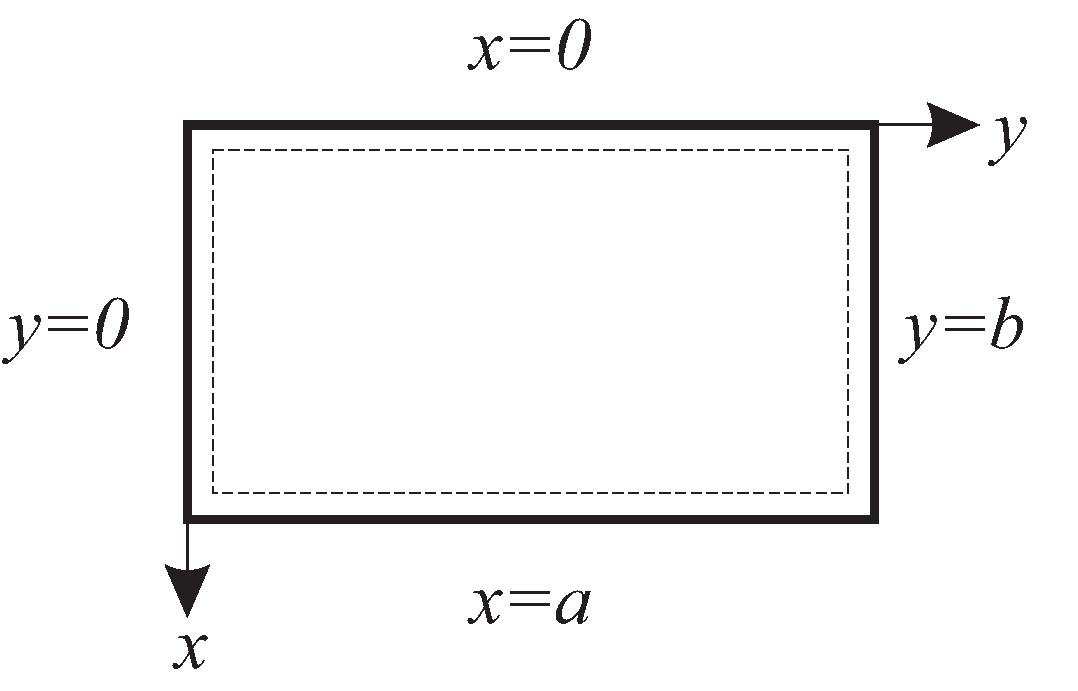
\includegraphics[width = 0.5\textwidth]{figures/ss_plate.pdf}
    \caption{The simply supported plate geometry and coordinate system}
    \label{fig:ss}
\end{figure}

Hence, the following boundary conditions are defined which meet the abovementioned initial boundary conditions \cite{Kant2002}.

\begin{flalign}
    & u_0 = \displaystyle\sum_{m = 1}^{\infty} \displaystyle\sum_{n = 1}^{\infty} u_{0mn} \cos(\alpha x) \sin(\beta y) \notag\\
    & u_1 = \displaystyle\sum_{m = 1}^{\infty} \displaystyle\sum_{n = 1}^{\infty} u_{1mn} \cos(\alpha x) \sin(\beta y) \notag\\
    & u_z = \displaystyle\sum_{m = 1}^{\infty} \displaystyle\sum_{n = 1}^{\infty} u_{zmn} \cos(\alpha x) \sin(\beta y) \notag\\
    & v_0 = \displaystyle\sum_{m = 1}^{\infty} \displaystyle\sum_{n = 1}^{\infty} v_{0mn} \sin(\alpha x) \cos(\beta y) \notag\\
    & v_1 = \displaystyle\sum_{m = 1}^{\infty} \displaystyle\sum_{n = 1}^{\infty} v_{1mn} \sin(\alpha x) \cos(\beta y) \notag\\
    & v_z = \displaystyle\sum_{m = 1}^{\infty} \displaystyle\sum_{n = 1}^{\infty} u_{zmn} \sin(\alpha x) \cos(\beta y) \notag\\
    & w_0 = \displaystyle\sum_{m = 1}^{\infty} \displaystyle\sum_{n = 1}^{\infty} w_{0mn} \sin(\alpha x) \sin(\beta y) 
    \label{eq:navier_Sol}
\end{flalign}

where $\alpha = m\pi/a$ and $\beta=n\pi/b$. $m$ and $n$ are positive integers which determine the number of terms for each double-Fourier series in \cref{eq:navier_Sol}. $a$ and $b$ are the plate length and width in $x$ and $y$-directions. \\

Based on the terms in \cref{eq:navier_Sol}, the transverse sinusoidal load is defined according to \cref{eq:navier_load}.

\begin{equation}
    q(x, y) = q_0 \sin(\alpha x) \sin(\beta b)
    \label{eq:navier_load}
\end{equation}

Substituting \cref{eq:navier_Sol} in \cref{eq:govern_eqn}, one is able to form the following system of equations 

\begin{equation}
    [\bm{K}]{\{\bm{d}}\} = \{\bm{p}\}
    \label{eq:sys_eq}
\end{equation}

in which $\bm{K}$ is a ($7\times7$) matrix and both $\bm{d}$ and $\bm{p}$ are column vectors of ($7\times1$) where 

\begin{flalign*}
    & \bm{d} = \{ u_0, u_1, u_z, v_0, v_1, v_z, w_0 \}^T \notag \\
    & \bm{p} = \{ 0, 0, 0 ,0 ,0 ,0 ,q(x, y) \}^T
\end{flalign*}

\subsection{The Solution Procedure}

\begin{figure}[!]
    \centering
    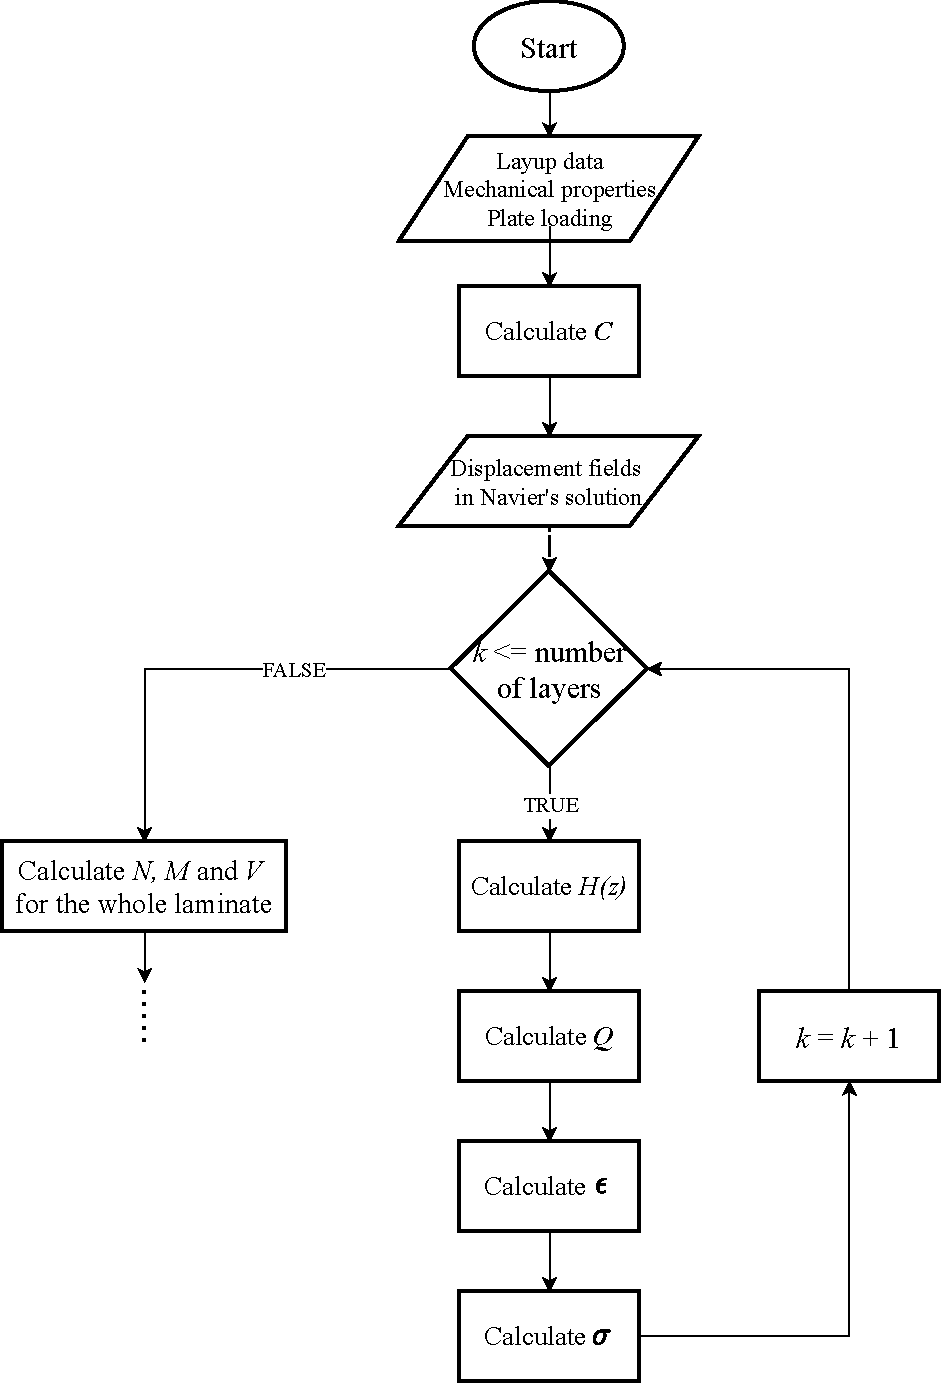
\includegraphics[width = 0.7\textwidth ]{figures/flowchart_matlab.pdf}
    \caption{The Navier's solution flowchart (MATLAB part). $k$ indicates the layer number.}
    \label{fig:flowchart_matlab}
\end{figure}

\begin{figure}[!]
    \centering
    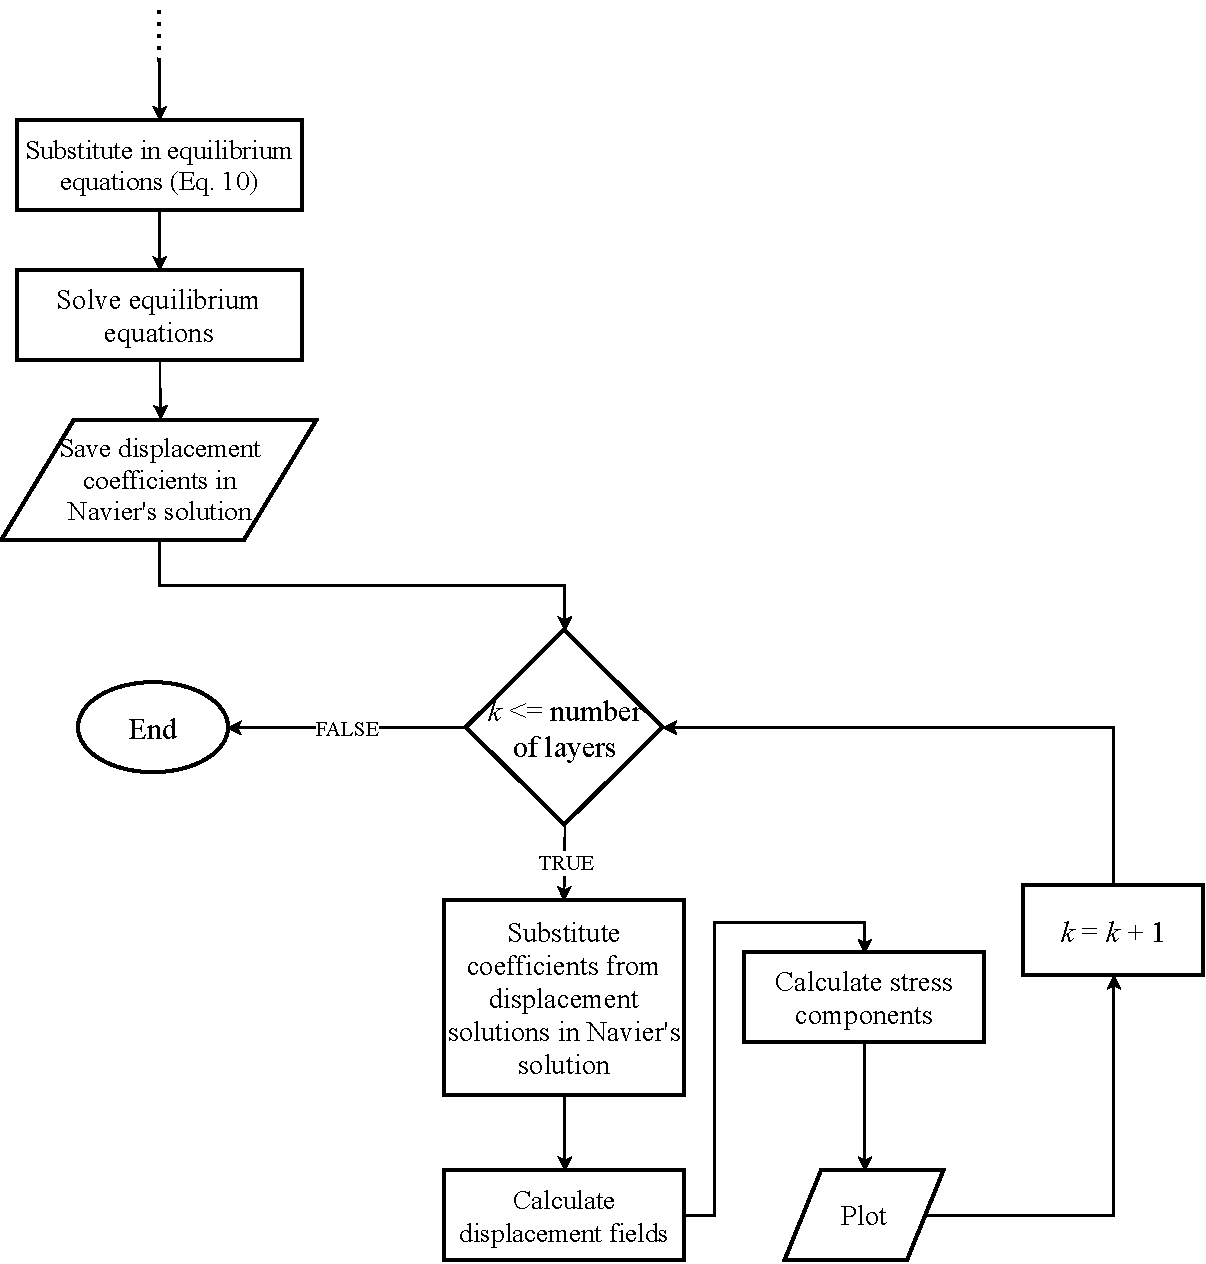
\includegraphics[width = 0.9\textwidth ]{figures/flowchart_maple.pdf}
    \caption{The Navier's solution flowchart (Maple part). $k$ indicates the layer number.}
    \label{fig:flowchart_maple}
\end{figure}

Codes are developed in both MATLAB and Maple\footnote{available on \url{github.com/amirbaharvand66/RSPTZ.git}}, which communicate through \texttt{.txt} files, to solve the given problem and the relevant flowcharts are provided in \cref{fig:flowchart_matlab} and \cref{fig:flowchart_maple}. The solution is performed for $m=1$ and $n=1$ in the double-Fourier series available in the Navier's solution. The precision of floating points in MATLAB and Maple are set to 16 and 10 digits, respectively. \\

The stacking layup of the composite laminate is [0/90/0] and mechanical properties are listed in \cref{tab:mech_prop}. The material is assumed to be transversely-isotropic ($E_{33}=E_{22}$, $\nu_{31} = \nu_{12}$ and $\mu_{31} = \mu_{12}$). Other constants can be found using \cref{eq:nu_componenst}.

\begin{table}[H]
\centering
\caption{Mechanical properties of the laminate.}
\begin{tabular}{lccc}
\hline
\textbf{Property}       & \textbf{Symbol}   & \textbf{Unit}   & \textbf{Value} \\ \hline
Longitudinal Young's modulus & $E_{11}$ & GPa & 172.5 \\
Transverse  Young's modulus & $E_{22}$ & GPa & 6.9 \\
In-plane Poisson's ratio & $\nu_{12}$ & - & 0.25 \\
Out-of-plane Poisson's ratio & $\nu_{23}$ & - & 0.25 \\
In-plane shear modulus & $\mu_{12}$ & GPa & 3.45 \\
Out-of-plane shear modulus & $\mu_{23}$ & GPa & 1.38 \\ \hline
\end{tabular}
\label{tab:mech_prop}
\end{table}

\subsection{Result and Discussion}
In addition to the present theory, Refined sinusoidal shear deformation plate theory including the zig-zag function (RSPTZ), two other codes including the Classical Laminate Plate Theory (CLPT) and the First-order Shear Deformation plate Theory (FSDT) are developed to provide a better comparison of the evaluated displacements and stresses by RSPTZ. One may, however; states that due to the thick geometrical aspect ratios ($a/h=4$ and $b/a=1$) of the plate under study, CLPT is inappropriate compared with the other two theories. CLPT is given for the sake of comparison and its effortless coding procedure. The results for the displacements and stresses are shown in \cref{fig:result} and are normalized using the equations in \cref{eq:norm_eqns}. In the current report, both $\tau_{xz}$ and $\tau_{yz}$ are not calculated from the three-dimensional elasticity solution.\\

As it can be seen, the RSPTZ by combining both sinusoidal shear deformation plate theory and zig-zag function is capable of showing the in-plane displacement (\cref{fig:sigma__xx_bar}) and its change of sign from one layer to another. For the thick plate, both CLPT and FSDT underestimate  $\overline{u}$, $\overline{\sigma}_{x}$, $\overline{\sigma}_{y}$ which is more pronounced on the free surfaces and interlaminar sections. CLPT is not capable of calculating $\tau_{xz}$ and $\tau_{yz}$, because of the assumptions in Kirchhoff's plate theory. As mentioned earlier, the determination of transverse stresses is absolutely-essential during the design level of composite structures. While the FSDT shows a constant distribution of $\tau_{xz}$ and $\tau_{yz}$ through each layer, that is due to the shear correction factor (here 5/6), RSPTZ can provide a nonlinear distribution of the aforementioned parameters throughout each individual layer. Furthermore, the zero transverse traction is also fulfilled using the RSPTZ on the top and bottom part of the laminate (\cref{fig:tau__xz_bar} and \cref{fig:tau__yz_bar}). 

\begin{equation}
\begin{matrix}
    \overline{u} = \dfrac{E_{22} h^2}{a^3} u \left (0, \dfrac{b}{2}, z\right ) \quad, \quad 
    \overline{w} = \dfrac{100 E_{22} h^3}{q_0 a^4} w \left (\dfrac{a}{2}, \dfrac{b}{2}, z\right ) \quad, \quad
    \overline{\sigma}_{x} = \dfrac{h^2}{q_0 a^2} \sigma_{x} \left (\dfrac{a}{2}, \dfrac{b}{2}, z\right )\\
    \overline{\sigma}_{y} = \dfrac{h^2}{q_0 a^2} \sigma_{y} \left (\dfrac{a}{2}, \dfrac{b}{2}, z\right ) \quad, \quad
    \overline{\tau}_{xy} = \dfrac{h^2}{q_0 a^2} \tau_{xy} \left (0, 0, z\right ) \quad, \quad
    \overline{\tau}_{xz} = \dfrac{h}{q_0 a} \tau_{xz} \left (0, \dfrac{b}{2}, z\right )\\
    \overline{\tau}_{yz} = \dfrac{h}{q_0 a} \tau_{yz}\left ( \dfrac{a}{2}, 0, z\right )
\end{matrix}
\label{eq:norm_eqns}
\end{equation}

\begin{figure}[!]
        \begin{subfigure}{0.5\textwidth}
            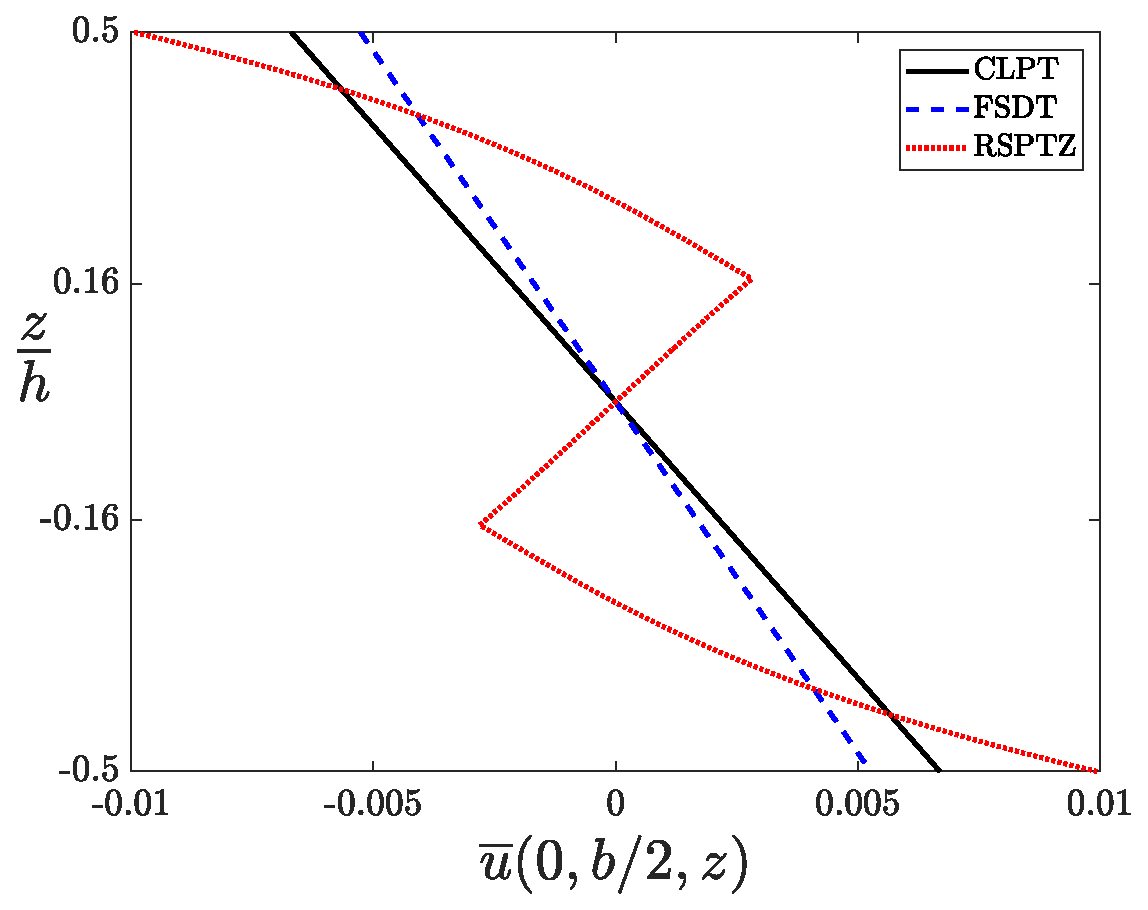
\includegraphics[width=1\linewidth, height=0.8\linewidth]{figures/u_bar.eps} 
            \caption{}
            \label{fig:u_bar}
        \end{subfigure}
        \begin{subfigure}{0.5\textwidth}
            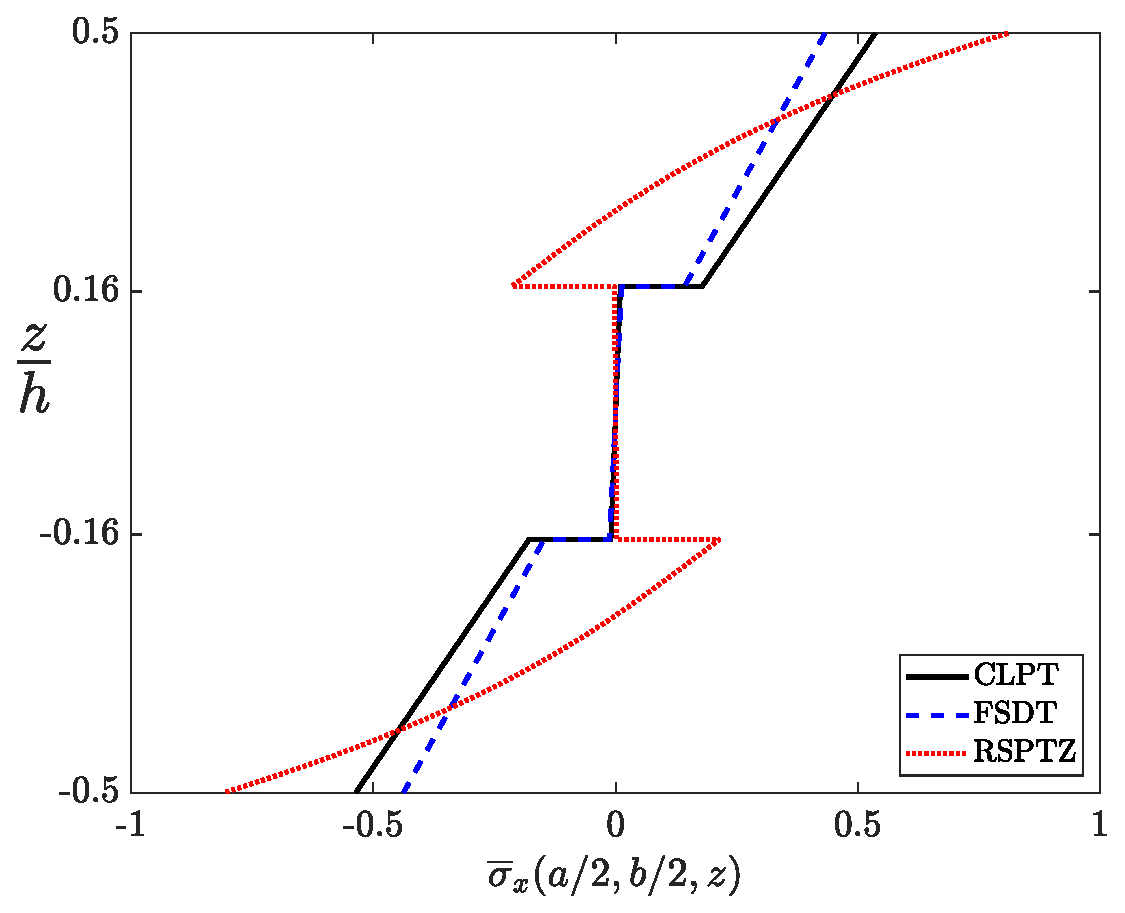
\includegraphics[width=1\linewidth, height=0.8\linewidth]{figures/sigma__xx_bar.eps} 
            \caption{}
            \label{fig:sigma__xx_bar}
        \end{subfigure}

        \begin{subfigure}{0.5\textwidth}
            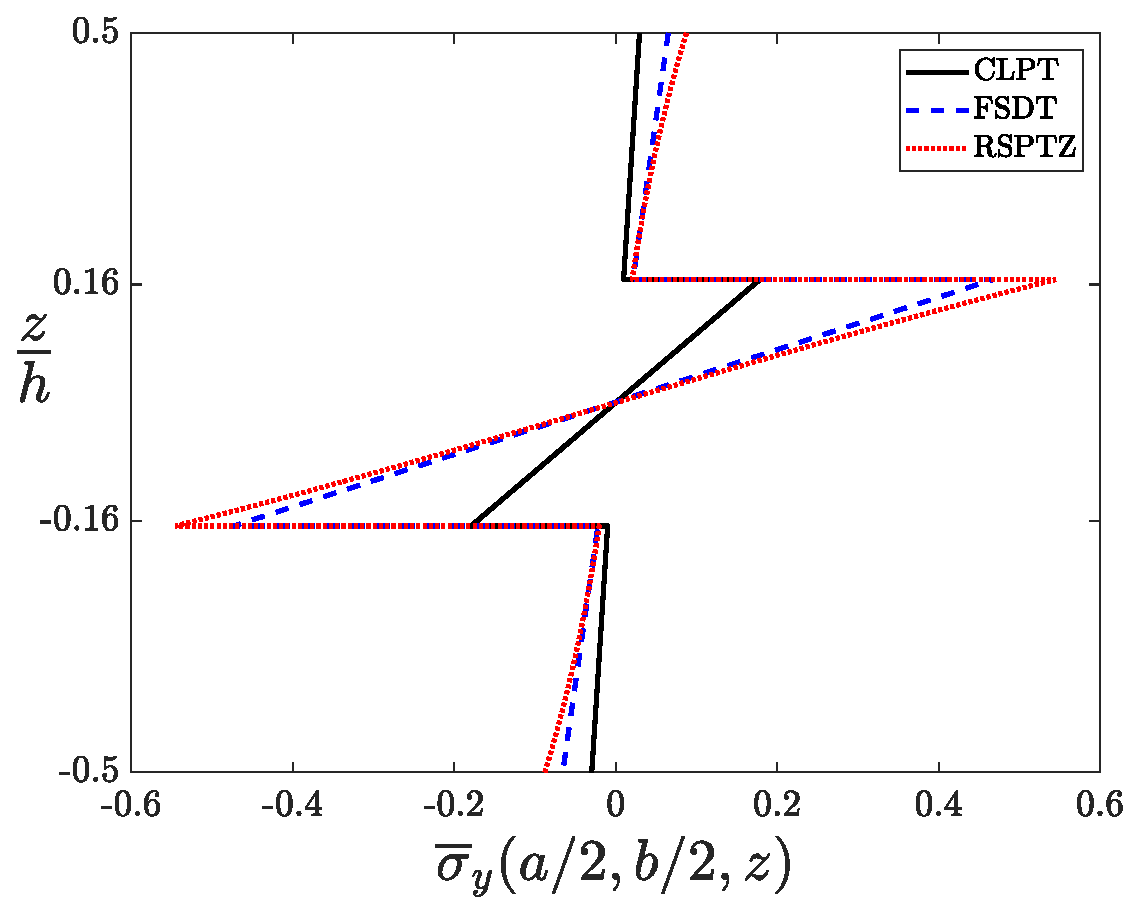
\includegraphics[width=1\linewidth, height=0.8\linewidth]{figures/sigma__yy_bar.eps} 
            \caption{}
            \label{fig:sigma__yy_bar}
        \end{subfigure}
        \begin{subfigure}{0.5\textwidth}
            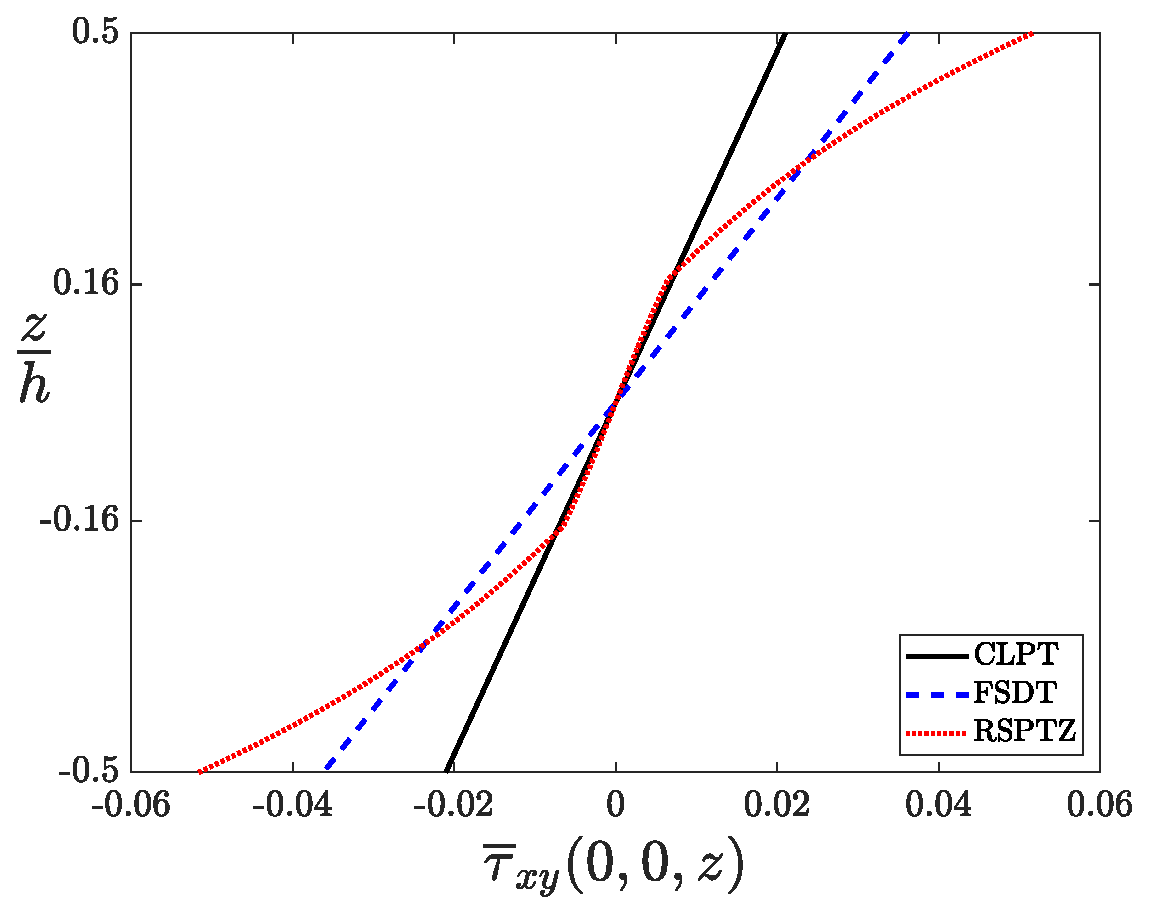
\includegraphics[width=1\linewidth, height=0.8\linewidth]{figures/tau__xy_bar.eps} 
            \caption{}
            \label{fig:tau__xy_bar}
        \end{subfigure}
    
        \begin{subfigure}{0.5\textwidth}
            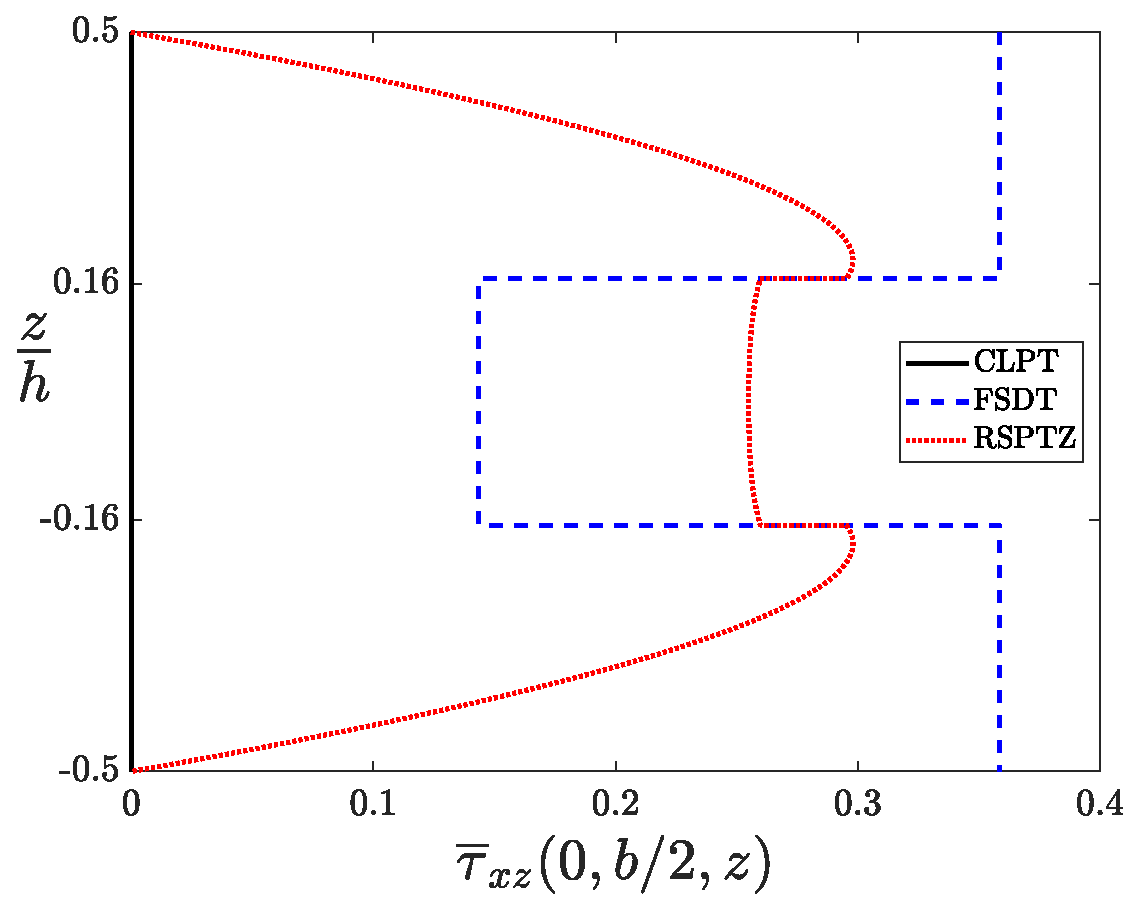
\includegraphics[width=1\linewidth, height=0.8\linewidth]{figures/tau__xz_bar.eps} 
            \caption{}
            \label{fig:tau__xz_bar}
        \end{subfigure}
        \begin{subfigure}{0.5\textwidth}
            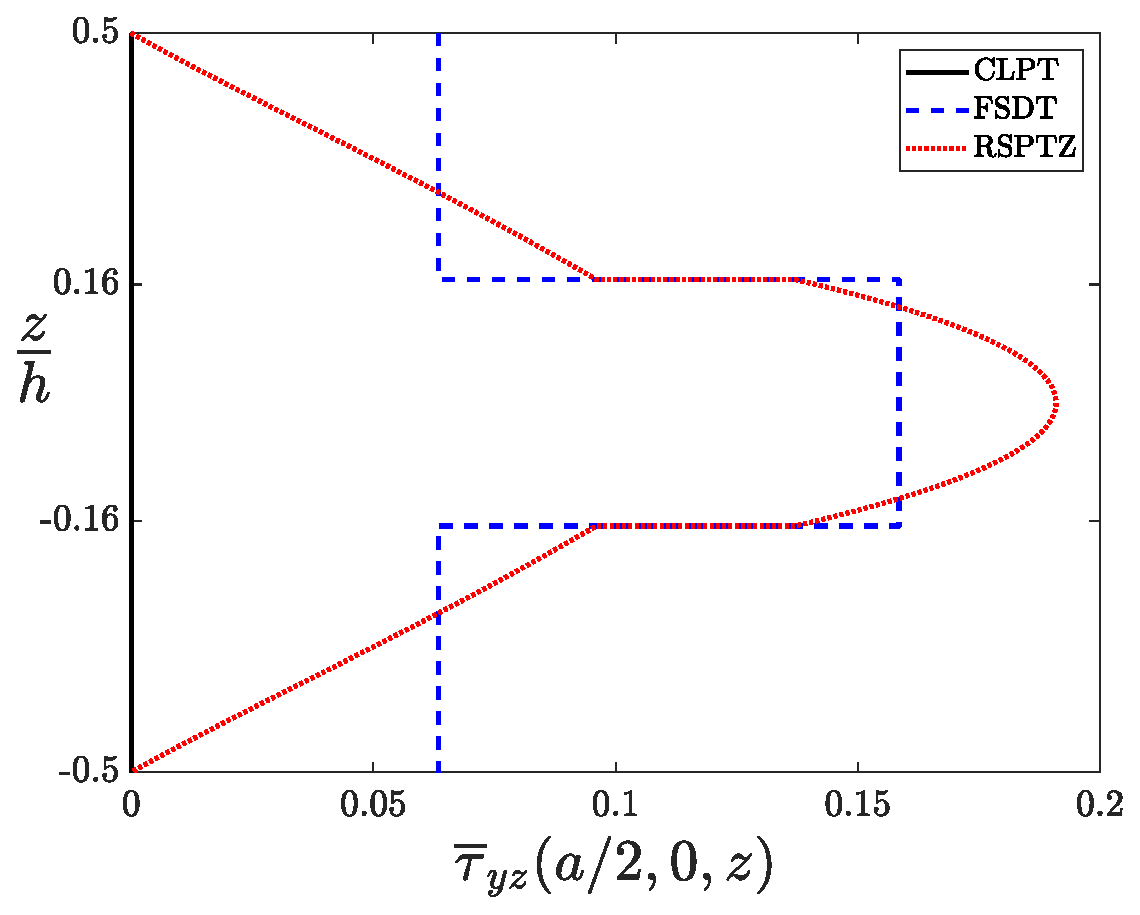
\includegraphics[width=1\linewidth, height=0.8\linewidth]{figures/tau__yz_bar.eps} 
            \caption{}
            \label{fig:tau__yz_bar}
        \end{subfigure}
    \caption{Comparison of normalized displacement and stress plots for a three-layer composite ([0, 90, 0]) under double sinusoidal load ($a/h=4$ and $b/a=1$). $\tau_{xz}$ and $\tau_{yz}$ are not calculated from the three-dimensional elasticity solution.}
    \label{fig:result}
\end{figure}

To provide a better insight into the present theory, RSPTZ is benchmarked against the exact solution from the three-dimensional elasticity solution by Pagano \cite{Pagano1969}. The result is summarized in \cref{tab:3d_elast_cmp}. The last two rows include the integrated values of $\tau_{xz}$ and $\tau_{yz}$ along the thickness.

\begin{table}[H]
\centering
\caption{Comparison of normalized displacement and stress for a three-layer composite ([0, 90, 0]) under double sinusoidal load ($a/h=4$ and $b/a=1$). Numbers in parentheses are the absolute error [\%] from the exact three-dimensional elasticity solution.}
\begin{tabular}{lcccc}
\hline
\textbf{Parameter} & \textbf{Exact} & \textbf{RSPTZ} & \textbf{FSDT} & \textbf{CLPT}\\ \hline
$\overline{u}(-h/2)$ & - & 0.0100 & 0.0050 & 0.0070 \\
$\overline{w}(0)$ & 2.006 & 2.0120(0.3) & 1.7620(12.2) & 0.4260(78.8) \\
$\overline{\sigma}_{x}(h/2)$ & 0.801 & 0.8090(1.0) & 0.4320(46.0) & 0.5360(33.1) \\
$\overline{\sigma}_{y}(h/6)$ & 0.534 & 0.5450(2.1) & 0.4680(12.4) & 0.1790(66.6) \\
$\overline{\tau}_{xy}(h/2)$ & 0.0505 & 0.0520(2.2) & 0.0360(28.3) & 0.0210(58.4) \\
$\overline{\tau}_{xz}(0)$ & 0.256 & 0.2550(0.4) & 0.1430(44.0) & 0(100) \\
$\overline{\tau}_{yz}(0)$ & 0.217 & 0.1910(12.0) & 0.1590(27.0) & 0(100) \\
$\int\overline{\tau}_{xz}$ & - & 0.2190(14.6) & 0.0720(72.0) & 0(100) \\
$\int\overline{\tau}_{yz}$ & - & 0.0900(58.5) & 0.0320(85.4) & 0(100) \\ \hline
\end{tabular}
\label{tab:3d_elast_cmp}
\end{table}

As expected, the results from CLPT are not satisfying and the FSDT gives a high-value error. Conversely, the RSPTZ is able to keep the error under 2\% except for $\overline{\tau}_{yz}$ where the error increases to 12\%. It also appears that the RSPTZ underestimates $\tau_{yz}$ if three-dimensional elasticity equations are not utilized.

\section{Conclusion}
Determination of the in-plane displacement and shear stress in laminate composites is vital during the design procedure. Therefore, new zig-zag method is presented which is capable of characterizing the zig-zag behavior of the displacement fields through the laminate thickness that has not been fulfilled by previously proposed sinusoidal theories. A priori traction free on the bottom and top surfaces of the laminate is another advantage of the present theory compared to the other zig-zag theories, \emph{i.e.}, Murakami's zig-zag theory. Displacements and stress components can be accurately calculated; nevertheless, it looks that the accuracy of the in-plane transverse stress falls without using the three-dimensional elasticity equations. 

\appendix
\section*{Appendices}
\section{Derivation of \texorpdfstring{$\delta U$}{} and \texorpdfstring{$\delta W$}{}} 

\subsection{Derivation of \texorpdfstring{$\delta U$}{}} \label{app:delU}

% \begin{flalign*}
%   & a = b & \\
%   & c = b &
% \end{flalign*}

% \begin{flalign}
%     \lambda &= \lambda_1 + \lambda_2 &\notag\\
%       &= \Lambda &\\
%       &= \Lambda_1 + \Lambda_2 & \notag
%  \end{flalign}

\begin{flalign*}
    & N_x \delta u_{0, x} = (N_x \delta u_0)_{,x} - N_{x, x} \delta u_0 & \\
    & M_{x1} \delta u_{1, x} = (M_{x1} \delta u_1)_{,x} - M_{x1, x} \delta u_1 & \\
    & M_{x2} \delta u_{z, x} = (M_{x2} \delta u_z)_{,x} - M_{x2, x} \delta u_z & \\
    & M_{x3} \delta w_{0, xx} = (M_{x3} \delta w_{0, x})_{,x} - M_{x3, x} \delta w_{0, x} =
    (M_{x3} \delta w_{0, x})_{,x} - (M_{x3, x} \delta w_0)_{,x} + M_{x3, xx} \delta w_0 & 
\end{flalign*}

\begin{flalign*}
    & N_y \delta v_{0, y} = (N_y \delta v_0)_{,y} - N_{y, y} \delta v_0 & \\
    & M_{y1} \delta v_{1, y} = (M_{y1} \delta v_1)_{,y} - M_{y1, y} \delta v_1 & \\
    & M_{y2} \delta v_{z, y} = (M_{y2} \delta v_z)_{,y} - M_{y2, y} \delta v_z & \\
    & M_{y3} \delta w_{0, yy} = (M_{y3} \delta w_{0, y})_{,y} - M_{y3, y} \delta w_{0, y} = 
    (M_{y3} \delta w_{0, y})_{,y} - (M_{y3, y} \delta w_0)_{,y} + M_{y3, yy} \delta w_0 &
\end{flalign*}

\begin{flalign*}
    & N_{xy} \delta u_{0, y} = (N_xy \delta u_0)_{,y} - N_{xy, y} \delta u_0 & \\
    & M_{xy1} \delta u_{1, y} = (M_{xy1} \delta u_1)_{,y} - M_{xy1, y} \delta u_1 & \\
    & M_{xy2} \delta u_{z, y} = (M_{xy2} \delta u_z)_{,y} - M_{xy2, y} \delta u_z & \\
    & M_{xy} \delta u_{0, x} = (N_xy \delta v_0)_{,x} - N_{xy, x} \delta v_0 & \\
    & M_{xy1} \delta v_{1, x} = (M_{xy1} \delta v_1)_{,x} - M_{xy1, x} \delta v_1 & \\
    & M_{xy2} \delta v_{z, x} = (M_{xy2} \delta v_z)_{,x} - M_{xy2, x} \delta v_z & \\
    & 2M_{xy3} \delta w_{0, xy} = 2[(M_{xy3} \delta w_{0, x})_{,y} - M_{xy3, y} \delta w_{0, x}] = 
    2[ (M_{xy3} \delta w_{0, x})_{,y} - (M_{xy3, y} \delta w_0)_{,x} + M_{xy3,xy} \delta w_0] &
\end{flalign*}


\begin{flalign}
    \int_{\Omega}^{} & \Bigg( \Bigg. - N_{x, x} \delta u_0 - M_{x1, x} \delta u_1 - M_{x2, x} \delta u_z + M_{x3, xx} \delta w_0 &\notag \\
     & - N_{y, y} \delta v_0 - M_{y1, y} \delta v_1 - M_{y2, y} \delta v_z + M_{y3, yy} \delta w_0 &\notag \\
     & + V_{y1} \delta v_1 + V_{y2} \delta v_z + V_{x1} \delta u_1 + V_{x2} \delta u_z &  &\notag\\
     & - N_{xy, y} \delta u_0 - M_{xy1, y} \delta u_1 - M_{xy2, y} \delta u_z &\notag \\
     & - N_{xy, x} \delta v_0 - M_{xy1, x} \delta v_1 - M_{xy2, x} \delta v_z &\notag \\
     & + 2M_{xy3,xy} \delta w_0 \Bigg. \Bigg) dxdy &
\end{flalign}

\begin{flalign}
    \int_{\Gamma}^{} & \Bigg( \Bigg. N_x n_x \delta u_0 + M_{x1} n_x \delta u_1 + M_{x2} n_x \delta u_z+ M_{x3} n_x \delta w_{0, x} - M_{x3, x} n_x \delta w_0  &\notag\\
    & + N_y n_y \delta v_0 + M_{y1} n_y \delta v_1 + M_{y2} n_y \delta v_z + M_{y3} n_y \delta w_{0, y} + M_{y3} n_y \delta w_{0, y} - M_{y3, y} n_y  &\notag\\
    & + N_xy n_y \delta u_0 + M_{xy1} n_y \delta u_1 + M_{xy2} n_y \delta u_z +
    N_xy n_x \delta v_0 + M_{xy1} n_x \delta v_1 + M_{xy2} n_x \delta v_z  &\notag\\
    & + 2M_{xy3} n_y \delta w_{0, x} - 2M_{xy3, y} n_x \delta w_0 \delta w_0 \Bigg. \Bigg) ds =  &\notag\\
    \int_{\Gamma}^{} & \Bigg( \Bigg. N_x n_x \delta u_0 + M_{x1} n_x \delta u_1 + M_{x2} n_x \delta u_z+ M_{x3} n_x \delta w_{0, x} - M_{x3, x} n_x \delta w_0  &\notag\\
    & + N_y n_y \delta v_0 + M_{y1} n_y \delta v_1 + M_{y2} n_y \delta v_z + M_{y3} n_y \delta w_{0, y} + M_{y3} n_y \delta w_{0, y} - M_{y3, y} n_y \delta w_0  &\notag\\
    & + N_xy n_y \delta u_0 + M_{xy1} n_y \delta u_1 + M_{xy2} n_y \delta u_z +
    N_xy n_x \delta v_0 + M_{xy1} n_x \delta v_1 + M_{xy2} n_x \delta v_z  &\notag\\
    & + 2M_{xy3} n_y \delta w_{0, x} - M_{xy3,y} n_x \delta w_0 - M_{xy3, x} n_y \delta w_0 \Bigg. \Bigg) ds &
\end{flalign}


where $M_{xy3} n_y \delta w_{0, x}$ vanishes in boundary conditions as the normal vector is $n = (0, 1)$ on planes $\delta w_{0, x}(x_0, y)$ and $\delta w_{0, x}(x_a, y)$.

\subsection{Derivation of \texorpdfstring{$\delta W$}{}} \label{app:delW}
% W_{px}

\begin{flalign*}
    & \delta u_z^1 = H^1(z) u_z = N^1(z) + N^1_1(z) + N^1_N(z)  & \\
    & N^1(z) = (-1)^1 \sinh(\zeta_1) & \\
    & N^1_1(z) = -(z^2 / 2 / z_1 + (z^3 -1.5z_1 z^2) / 6 / z^2_{2})(-a_1\cosh(-1)) & \\
    & N^1_N(z) = -((z^3 - 1.5z_1 z^2) / 6 / z^2_{2})((-1)^1 a_1 \cosh(1)) & \\
    & \zeta_1 = a_1 z - b_1 , a_1 = \frac{2}{z_{2} - z_1} , b_1 = \frac{z_{2} + z_1}{z_{2} - z_1} &
\end{flalign*}

\begin{flalign*}
    & \delta u_z^N = H^N(z) u_z = N^N(z) + N^N_1(z) + N^N_N(z)  & \\
    & N^N(z) = (-1)^N \sinh(\zeta_N) & \\
    & N^N_1(z) = -(z^2 / 2 / z_1 + (z^3 -1.5z_1 z^2) / 6 / z^2_{N+1})(-a_1\cosh(-1)) & \\
    & N^N_N(z) = -((z^3 - 1.5z_1 z^2) / 6 / z^2_{N+1})((-1)^N a_N \cosh(1)) & \\
    & \zeta_N = a_N z - b_N , a_N = \frac{2}{z_{N+1} - z_N} , b_N = \frac{z_{N+1} + z_N}{z_{N+1} - z_N} &
\end{flalign*}

\begin{flalign*}
    \delta W_{px} = -\int_{\Omega} & \Bigg( \Bigg. p_x^b \delta u_0 + \phi_3^1 p_x^b \frac{\partial \delta w_0}{\partial x} + \phi_1^1 p_x^b \delta u_1 + \phi_2^1 p_x^b \delta u_z   &\notag \\
     & + p_x^t \delta u_0 + \phi_3^N p_x^t \frac{\partial \delta w_0}{\partial x} + \phi_1^N p_x^t \delta u_1 + \phi_2^N p_x^t \delta u_z \Bigg. \Bigg) &\notag \\
    = -\int_{\Omega} & \Bigg( \Bigg. \{p_x^b + p_x^t\} \delta u_0 + \{\phi_3^1 p_x^b +\phi_3^N p_x^t \} \frac{\partial \delta w_0}{\partial x}  \delta u_z &\notag \\
     & + \{\phi_1^1 p_x^b + \phi_1^N p_x^t \} \delta u_1 + \{\phi_2^1 p_x^b +\phi_2^N p_x^t \} \Bigg. \Bigg) dxdy = &\notag \\
\end{flalign*}

where

\begin{flalign*}
    & p_{x_0} = p_x^b + p_x^t  & \\
    & p_{x_1} = \phi_2^1 p_x^b +\phi_2^N p_x^t & \\
    & p_{x_2} = \phi_1^1 p_x^b + \phi_1^N p_x^t & \\
    & p_{x_3} = \phi_3^1 p_x^b +\phi_3^N p_x^t & 
\end{flalign*}

% W_{py}
\begin{flalign*}
    & \delta v_z^1 = H^1(z) v_z = N^1(z) + N^1_1(z) + N^1_N(z)  & \\
    & N^1(z) = (-1)^1 \sinh(\zeta_1) & \\
    & N^1_1(z) = -(z^2 / 2 / z_1 + (z^3 -1.5z_1 z^2) / 6 / z^2_{2})(-a_1\cosh(-1)) & \\
    & N^1_N(z) = -((z^3 - 1.5z_1 z^2) / 6 / z^2_{2})((-1)^1 a_1 \cosh(1)) & \\
    & \zeta_1 = a_1 z - b_1 , a_1 = \frac{2}{z_{2} - z_1} , b_1 = \frac{z_{2} + z_1}{z_{2} - z_1} &
\end{flalign*}

\begin{flalign*}
    & \delta v_z^N = H^N(z) v_z = N^N(z) + N^N_1(z) + N^N_N(z)  & \\
    & N^N(z) = (-1)^N \sinh(\zeta_N) & \\
    & N^N_1(z) = -(z^2 / 2 / z_1 + (z^3 -1.5z_1 z^2) / 6 / z^2_{N+1})(-a_1\cosh(-1)) & \\
    & N^N_N(z) = -((z^3 - 1.5z_1 z^2) / 6 / z^2_{N+1})((-1)^N a_N \cosh(1)) & \\
    & \zeta_N = a_N z - b_N , a_N = \frac{2}{z_{N+1} - z_N} , b_N = \frac{z_{N+1} + z_N}{z_{N+1} - z_N} &
\end{flalign*}

\begin{flalign*}
    \delta W_{py} = -\int_{\Omega} & \Bigg( \Bigg. p_y^b \delta v_0 + \phi_3^1 p_y^b \frac{\partial \delta w_0}{\partial y} + \phi_1^1 p_y^b \delta v_1 + \phi_2^1 p_y^b \delta v_z   &\notag \\
     & + p_y^t \delta v_0 + \phi_3^N p_y^t \frac{\partial \delta w_0}{\partial y} + \phi_1^N p_y^t \delta v_1 + \phi_2^N p_y^t \delta v_z \Bigg. \Bigg) &\notag \\
    = -\int_{\Omega} & \Bigg( \Bigg. \{p_y^b + p_y^t\} \delta v_0 + \{\phi_3^1 p_y^b +\phi_3^N p_y^t \} \frac{\partial \delta w_0}{\partial y}  \delta v_z &\notag \\
     & + \{\phi_1^1 p_y^b + \phi_1^N p_y^t \} \delta v_1 + \{\phi_2^1 p_y^b +\phi_2^N p_y^t \} \Bigg. \Bigg) dydy = &\notag \\
\end{flalign*}

where

\begin{flalign*}
    & p_{y_0} = p_y^b + p_y^t  & \\
    & p_{y_1} = \phi_2^1 p_y^b +\phi_2^N p_y^t & \\
    & p_{y_2} = \phi_1^1 p_y^b + \phi_1^N p_y^t & \\
    & p_{y_3} = \phi_3^1 p_y^b +\phi_3^N p_y^t & 
\end{flalign*}

    
\begin{flalign*}
    &\delta W_{q} = -\int_{\Omega} ( q^b \delta w_0 + q^t \delta w_0 ) dxdy = -\int_{\Omega} ( q^b + q^t) \delta w_0 dxdy = -\int_{\Omega} (q \delta w_0) dxdy &\notag
\end{flalign*}

\begin{flalign*}
    \delta W_{Tx0} & = -\int_{-\frac{h}{2}}^{\frac{h}{2}} \left [ T_{x_0} \delta u^k (x_0, y, z) + T_{xz0} \delta w(x_0, y, z) \right ] dz &\notag \\
    & = -\int_{-\frac{h}{2}}^{\frac{h}{2}} \left [ T_{x_0} \delta u_0 + \phi_3 T_{x_0} \frac{\partial \delta w_0}{\partial x} + \phi_1 T_{x_0} + \phi_2 T_{x_0} + T_{xz0} \delta w_0 \right ] dz & 
\end{flalign*}

\begin{flalign*}
    \delta W_{Ty0} & = -\int_{-\frac{h}{2}}^{\frac{h}{2}} \left [ T_{y_0} \delta v^k (y_0, y, z) + T_{yz0} \delta w(y_0, y, z) \right ] dz &\notag \\
    & = -\int_{-\frac{h}{2}}^{\frac{h}{2}} \left [ T_{y_0} \delta v_0 + \phi_3 T_{y_0} \frac{\partial \delta w_0}{\partial y} + \phi_1 T_{y_0} + \phi_2 T_{y_0} + T_{yz0} \delta w_0 \right ] dz & 
\end{flalign*}

\begin{flalign*}
    \delta W_{Txa} & = -\int_{-\frac{h}{2}}^{\frac{h}{2}} \left [ T_{x_a} \delta u^k (x_a, y, z) + T_{xza} \delta w(x_a, y, z) \right ] dz &\notag \\
    & = -\int_{-\frac{h}{2}}^{\frac{h}{2}} \left [ T_{x_a} \delta u_a + \phi_3 T_{x_a} \frac{\partial \delta w_0}{\partial x} + \phi_1 T_{x_a} + \phi_2 T_{x_a} + T_{xza} \delta w_0 \right ] dz & 
\end{flalign*}

\begin{flalign*}
    \delta W_{Tyb} & = -\int_{-\frac{h}{2}}^{\frac{h}{2}} \left [ T_{y_b} \delta v^k (y_b, y, z) + T_{yzb} \delta w(y_b, y, z) \right ] dz &\notag \\
    & = -\int_{-\frac{h}{2}}^{\frac{h}{2}} \left [ T_{y_b} \delta v_b + \phi_3 T_{y_b} \frac{\partial \delta w_0}{\partial y} + \phi_1 T_{y_b} + \phi_2 T_{y_b} + T_{yzb} \delta w_0 \right ] dz & 
\end{flalign*}

where

\begin{equation}
\begin{matrix}
    \begin{Bmatrix}
            \overline{N}_{x0} \\
            \overline{M}_{x10} \\
            \overline{M}_{x20} \\
            \overline{M}_{x30} \\
    \end{Bmatrix} = 
    \displaystyle\int_{-\frac{h}{2}}^{\frac{h}{2}}
    \begin{Bmatrix}
            T_{x0} \\
            \phi_1 T_{x0} \\
            \phi_2 T_{x0} \\
            \phi_3 T_{x0} \\
    \end{Bmatrix}
    dz,
    \begin{Bmatrix}
            \overline{N}_{y0} \\
            \overline{M}_{y10} \\
            \overline{M}_{y20} \\
            \overline{M}_{y30} \\
    \end{Bmatrix} = 
    \displaystyle\int_{-\frac{h}{2}}^{\frac{h}{2}}
    \begin{Bmatrix}
            T_{y0} \\
            \phi_1 T_{y0} \\
            \phi_2 T_{y0} \\
            \phi_3 T_{y0} \\
    \end{Bmatrix}
    dz
\end{matrix}
\label{eq:bc_Bar_terms1}
\end{equation}

\begin{equation}
\begin{matrix}
    \begin{Bmatrix}
            \overline{N}_{xa} \\
            \overline{M}_{x1a} \\
            \overline{M}_{x2a} \\
            \overline{M}_{x3a} \\
    \end{Bmatrix} = 
    \displaystyle\int_{-\frac{h}{2}}^{\frac{h}{2}}
    \begin{Bmatrix}
            T_{x0} \\
            \phi_1 T_{xa} \\
            \phi_2 T_{xa} \\
            \phi_3 T_{xa} \\
    \end{Bmatrix}
    dz,
    \begin{Bmatrix}
            \overline{N}_{yb} \\
            \overline{M}_{y1b} \\
            \overline{M}_{y2b} \\
            \overline{M}_{y3b} \\
    \end{Bmatrix} = 
    \displaystyle\int_{-\frac{h}{2}}^{\frac{h}{2}}
    \begin{Bmatrix}
            T_{y0} \\
            \phi_1 T_{yb} \\
            \phi_2 T_{yb} \\
            \phi_3 T_{yb} \\
    \end{Bmatrix}
    dz
\end{matrix}
\label{eq:bc_Bar_terms2}
\end{equation}

\begin{equation}
\begin{matrix}
    \begin{Bmatrix}
            \overline{V}_{xz0} \\
            \overline{V}_{yz0} \\
    \end{Bmatrix} = 
    \displaystyle\int_{-\frac{h}{2}}^{\frac{h}{2}}
    \begin{Bmatrix}
            T_{xz0} \\
            T_{yz0} \\
    \end{Bmatrix}
    dz,
    \begin{Bmatrix}
            \overline{V}_{xza} \\
            \overline{V}_{yzb} \\
    \end{Bmatrix} = 
    \displaystyle\int_{-\frac{h}{2}}^{\frac{h}{2}}
    \begin{Bmatrix}
            T_{xza} \\
            T_{yzb} \\
    \end{Bmatrix}
    dz
\end{matrix}
\label{eq:bc_Bar_terms3}
\end{equation}
\section{Components of \texorpdfstring{$\boldsymbol{Q}$}{}} \label{app:stiff_mat}
\subsection{Components of \texorpdfstring{$\boldsymbol{C}$}{}}
$\bm{C}$ is the stiffness matrix and is defined according to each lay-up coordinate system (1, 2, 3). 

\begin{equation}
\begin{Bmatrix}
\sigma_1\\ 
\sigma_2\\ 
\sigma_3\\ 
\tau_{12}\\ 
\tau_{23}\\ 
\tau_{31}
\end{Bmatrix}
=\begin{bmatrix}
C_{11} & C_{12} & C_{13} & 0 & 0 & 0 \\ 
C_{12} & C_{22} & C_{23} & 0 & 0 & 0 \\ 
C_{13} & C_{23} & C_{33} & 0 & 0 & 0 \\ 
0 & 0 & 0 & C_{44} & 0 & 0 \\ 
0 & 0 & 0 & 0 & C_{55} & 0 \\ 
0 & 0 & 0 & 0 & 0 & C_{66}
\end{bmatrix}
\begin{Bmatrix}
\epsilon_1\\ 
\epsilon_2\\ 
\epsilon_3\\ 
\gamma_{12}\\ 
\gamma_{23}\\ 
\gamma_{31}
\end{Bmatrix}
\label{eq:C_mat}
\end{equation}

where the components of $\bm{C}$ are

\begin{equation*}
\begin{matrix}
    C_{11} = \displaystyle\frac{E_{11} (1 - \nu_{23} \nu_{32})}{\Delta} \quad, \quad
    C_{12} = \displaystyle\frac{E_{11} (\nu_{21} + \nu_{31} \nu_{23})}{\Delta} \quad, \quad
    C_{13} = \displaystyle\frac{E_{11} (\nu_{31} + \nu_{21} \nu_{32})}{\Delta}
\end{matrix}
\end{equation*}

\begin{equation*}
\begin{matrix}
    C_{22} = \displaystyle\frac{E_{22} (1 - \nu_{13} \nu_{31})}{\Delta} \quad , \quad
    C_{23} = \displaystyle\frac{E_{22} (\nu_{32} + \nu_{12} \nu_{31})}{\Delta} \quad, \quad
    C_{33} = \displaystyle\frac{E_{33} (1 - \nu_{12} \nu_{21})}{\Delta}
\end{matrix}
\end{equation*}

\begin{equation}
\begin{matrix}
    C_{44} = \mu_{12} \quad, \quad
    C_{55} = \mu_{23} \quad, \quad
    C_{66} = \mu_{13} \quad
\end{matrix}
\end{equation}

\begin{equation}
\begin{matrix}
    \Delta = 1 - \nu_{12} \nu_{21} - \nu_{23} \nu_{32} - \nu_{31} \nu_{13} - \nu_{21} \nu_{32} \nu_{13} - \nu_{12} \nu_{23} \nu_{31}
\end{matrix}
\label{eq:C_components}
\end{equation}

$E_{11}$ is the longitudinal Young's modulus, $E_{22}$ and $E_{33}$ are transverse Young's moduli, $\mu_{12}$ and $\mu_{13}$ are in-plane shear moduli, $\mu_{23}$ is the out-of-plane shear modulus, $\nu_{12}$ and $\nu_{13}$ are in-plane Poisson's ratios and $\nu_{23}$ is the out-of-plane Poisson's ratio. Other constants are calculated from the following set of equations.

\begin{equation}
\begin{matrix}
    \dfrac{\nu_{12}}{E_{11}} = \dfrac{\nu_{21}}{E_{22}} \quad , \quad
    \dfrac{\nu_{13}}{E_{11}} = \dfrac{\nu_{31}}{E_{33}} \quad , \quad
    \dfrac{\nu_{23}}{E_{22}} = \dfrac{\nu_{32}}{E_{33}}
\end{matrix}
\label{eq:nu_componenst}
\end{equation}

\subsection{Components of \texorpdfstring{$\boldsymbol{Q}$}{}}

\begin{flalign}
    & Q_{11} = C_{11} c^4 + 2 (C_{12} + 2 C_{44}) s^2 c^2 + C_{22} s^4& \notag \\
    & Q_{12} = C_{12} (c^4 + s^4) + (C_{11} + C_{22} - 4 C_{44}) s^2 c^2&  \notag \\
    & Q_{13} = C_{13} c^2 + C_{23} s^2 & \notag \\
    & Q_{14} = (C_{11} - C_{12} - 2 C_{44}) s c^3 + (C_{12} - C_{22} + 2 C_{44}) c s^3 & \notag \\
    & Q_{22} = C_{11} s^4 + C_{22} c^4 + (2 C_{12} + 4 C_{44}) s^2 c^2 & \notag \\
    & Q_{23} = C_{13} s^2 + C_{23} c^2 & \notag \\
    & Q_{24} = (C_{11} - C_{12} - 2 C_{44}) s^3 c + (C_{12} - C_{22} + 2 C_{44}) c^3 s & \notag \\
    & Q_{33} = C_{33} & \notag \\
    & Q_{34} = (C_{31} - C_{32}) s c & \notag \\
    & Q_{44} = (C_{11} - 2 C_{12} + C_{22} - 2 C_{44}) c^2 s^2 + C_{44} (c^4 + s^4) & \notag \\
    & Q_{55} = C_{55} c^2 + C_{66} s^2 & \notag \\
    & Q_{56} = (C_{66} - C_{55}) c s & \notag \\
    & Q_{66} = C_{55} s^2 + C_{66} c^2 & 
\end{flalign}

where $c = \cos(\theta)$, $s = \sin(\theta)$ and $Q_{ij} = Q_{ji}$ for $i, j = 1..6$



\newpage
\bibliography{ref}
\bibliographystyle{ieeetr}

\end{document}